% makeindex next2.idx
% License: GNU Free Documentation License 1.2.
\documentclass{jbook}
%\usepackage{html}
\usepackage{makeidx}
\usepackage{ascmac}
\usepackage[dvips]{graphicx}
\textwidth = 15cm
\textheight = 23cm

\topmargin = 0.7cm
\evensidemargin = 0cm
\oddsidemargin = 1cm

\def\comment#1{ #1 }
%\def\comment#1{  }
\newenvironment{FRAME}{\begin{trivlist}\item[]
  \hrule
  \hbox to \linewidth\bgroup
  \advance\linewidth by -30pt
  \hsize=\linewidth
  \vrule\hfill
  \vbox\bgroup
    \vskip15pt
    \def\thempfootnote{\arabic{mpfootnote}}
    \begin{minipage}{\linewidth}}{%
    \end{minipage}\vskip15pt
  \egroup\hfill\vrule
 \egroup\hrule
\end{trivlist}}

\newcommand{\yenn}{{\ooalign{Y\crcr\hss=\hss}}}
\def\blskip{\vskip\baselineskip}

%%%%%%%%%%%%%%%%%  macro definitions %%%%%%%%%%%%%%%%%%%%%
\def\QQQ{\fbox{{\bf 質問}}}
\def\AAA{{\fbox{\bf 答え}}}
\def\HHH{{\fbox{\bf 発展学習}}}
\newtheorem{problem}{\fbox{問題}}[chapter]
\newtheorem{answer}{答え}[chapter]
\newtheorem{program}{プログラム}[chapter]
\newtheorem{experiment}{実験}[chapter]
\newtheorem{example}{\fbox{例}}[chapter]
\newtheorem{exampleOutput}{出力例}[chapter]
\newtheorem{exampleInput}{入力例}[chapter]
\newtheorem{exampleInputOutput}{入出力例}[chapter]
\newtheorem{question}{疑問}[chapter]
\newtheorem{theorem}{定理}[chapter]
\newtheorem{remark}{注意}[chapter]
\newtheorem{algorithm}{アルゴリズム}[chapter]
\def\Begin{
  \rm
}
\def\END{
  \par \bigbreak
} 
\def\command#1{
 \fbox{\tt ALT}{\tt +}\fbox{\tt #1}
}
\def\alt#1{
 \fbox{\tt ALT}{\tt +}\fbox{\tt #1}
}
\def\shift#1{
 \fbox{\tt SHIFT}{\tt +}\fbox{\tt #1}
}
\def\command#1{
 \fbox{\tt COMMAND}{\tt +}\fbox{\tt #1}
}
\def\ctrl#1{
 \fbox{\tt CTRL}{\tt +}\fbox{\tt #1}
}
\def\esc#1{
 \fbox{\tt esc} \fbox{\tt #1}
}
\def\return{
 \fbox{\tt RETURN}
}
\def\expr{
 {\it expr}
}
\def\poly{
 {\it poly}
}
\def\f{
 {\it f}
}
\def\range{
 {\it \{ x, xmin, xmax \}}
}
\def\power{
\verb+^+}
\def\file{
 ファイル名
}


\title{ {\bf 超入門 Cfep/asir (MacOS X)} }
\author{  高山信毅 }
\date{ 2006年(平成18年), 3月12日版(cfep 1.1). 2008-09-26, 2009-09-19, 2012-08-28 修正 \\ コメントは takayama@math.kobe-u.ac.jp まで}
\makeindex

\begin{document}
\maketitle
\tableofcontents

\chapter{ 電卓としての利用 }  \label{chapter:next}
%en \chapter{A Tour of Asir} \label{chapter:next}

神戸大学の教育用計算機環境が MacOS X に変更されるのに伴い,
筆者が教材として利用していた Windows で動作する10進Basicが利用できなくなった.
Cfep/asir はその代用として, 
2006年初頭から開発を進めているシステムである.
10進Basicの優れている点の一つは, 丁寧な入門解説が付属していることである.
``Cfep/asir超入門'' はこの解説にすこしでも近付こうと努力してみた.
Asirの入門テキストに ``Asirドリル'' があるが, この超入門では ``Asirドリル''
の一章およびその先の入門的内容を丁寧に(少々くどく)説明した.

\bigbreak

この節では MacOS X での cfep/asir の起動法, 電卓風, Basic風の使い方を説明する.
ファイルの保存等 MacOS X の共通の操作方法にはほとんどふれていないが,
cfep/asir は MacOS X 標準のファイルの保存等を用いているので,
このような部分では他のソフトウエアと利用方法は同一である.
初心者の人は適当な本やガイドを参照されたい.


\section{キー操作と用語の復習}

\noindent
キーボード, マウスの操作の用語.
\begin{enumerate}
%
\item
 \fbox{\tt Command} キーや
 \fbox{\tt ALT } キーや \fbox{\tt SHIFT} キーや
 \fbox{\tt CTRL } キーは他のキーと一緒に押すことで始めて機能する
 キーである.これらだけを単独に押してもなにもおきない.
 以後 \fbox{\tt SHIFT} キーをおしながら他のキーを押す操作を
 \shift{きー} と書くことにする. command キー, alt キー,  ctrl キーについても 
 同様である.
%
\item
 \shift{a} とすると大文字の A を入力できる.
%
\item
 \fbox{\tt BS} とか \fbox{\tt DEL} と書いてあるキー押すと一文字前を消去できる.
%
\item 日本語キーボードの場合 \fbox{{\tt $\backslash$}}
(バックスラッシュ) は \alt{\yen} で入力できる.
%
\item
 \fbox{\tt SPACE} キーは空白を入力するキーである.
  計算機の内部では文字は数字に変換されて格納および処理される.
  文字に対応する数字を文字コードと呼ぶ. 文字コードにはいろいろな種類のものがあるが,
  一番基礎的なのはアスキーコード系であり, アルファベットや数字, キーボードに現れる
  記号などをカバーしている. 漢字はアスキーコード系では表現できない.
  \fbox{A} のアスキーコードは 65番である. 以下 \fbox{B} が 66, \fbox{C} が 67,
  と続く. 
  空白のアスキーコードは32番である.
 日本語入力の状態で入力される空白は ``全角空白'' と呼ばれており,
 アスキーコード32番の空白 (半角空白) とは別の文字である.
 全角空白がプログラムに混じっているとエラーを起こす.
 asir ではメッセージやコメント等に日本語が利用可能であるが, 
 慣れるまでは英字モードのみを利用することをお勧めする.
 右上の言語表示が 
\begin{center}
  \scalebox{0.1}{
\includegraphics{Figs/language.ps}} 
\end{center}
 となっている状態で cfep/asir に入力しよう.
% 
\item
 \fbox{  ' } (シングルクオート) と \fbox{ `  }  (バッククオート)
は別の文字である.
 プログラムを読む時に注意.
 また, プログラムを読む時は {\tt 0} (ゼロ)と {\tt o} (おー)
 の違いにも注意.
%
%
\item
 マウスの操作には次の三種類がある.
% 
%
\begin{enumerate}
\item クリック: 選択するとき, 
       文字を入力する位置(キャレットの位置)の移動に用いる.
      マウスのボタンをちょんとおす.  \index{くりっく@クリック}
\item ドラッグ: 移動, サイズの変更, 範囲の指定, コピーの
      ときなどに用いる.
      マウスのボタンを押しながら動かす.
\item ダブルクリック:プログラムの実行, open(ファイルを開く)をするために
      用いる.  \index{だぶるくりっく@ダブルクリック}
       マウスのボタンを2回つずけてちょんちょんとおす.
      ダブルクリックをしたアイコンは白くなったり形状がかわることが
      おおい.
      ダブルクリックしたらしばらく待つ.
      計算機が忙しいときは起動に時間がかかることもあり.
      むやみにダブルクリックを繰り返すとその回数だけ起動されてなお遅くなる.
\end{enumerate}
%
\end{enumerate}


\section{ Cfep/Asir の起動法と電卓的な使い方 }
%en \section{Using Risa/Asir as a Calculator}
%C

cfep のアイコン(いのぶた君)
%en
%en In case of Windows, open the folder (directory) in which Risa/Asir is
%en installed and double click the icon of {\tt asirgui}
%<C
\begin{center}
\scalebox{0.1}{
\includegraphics{Figs/inobuta.ps}}
\end{center}
%>C
をダブルクリックすると図\ref{fig:cfepStart}のように cfep/asir が起動する.
以下 cfep/asir を単に asir とよぶ.

%<C
\begin{figure}[tb]
\scalebox{0.5}{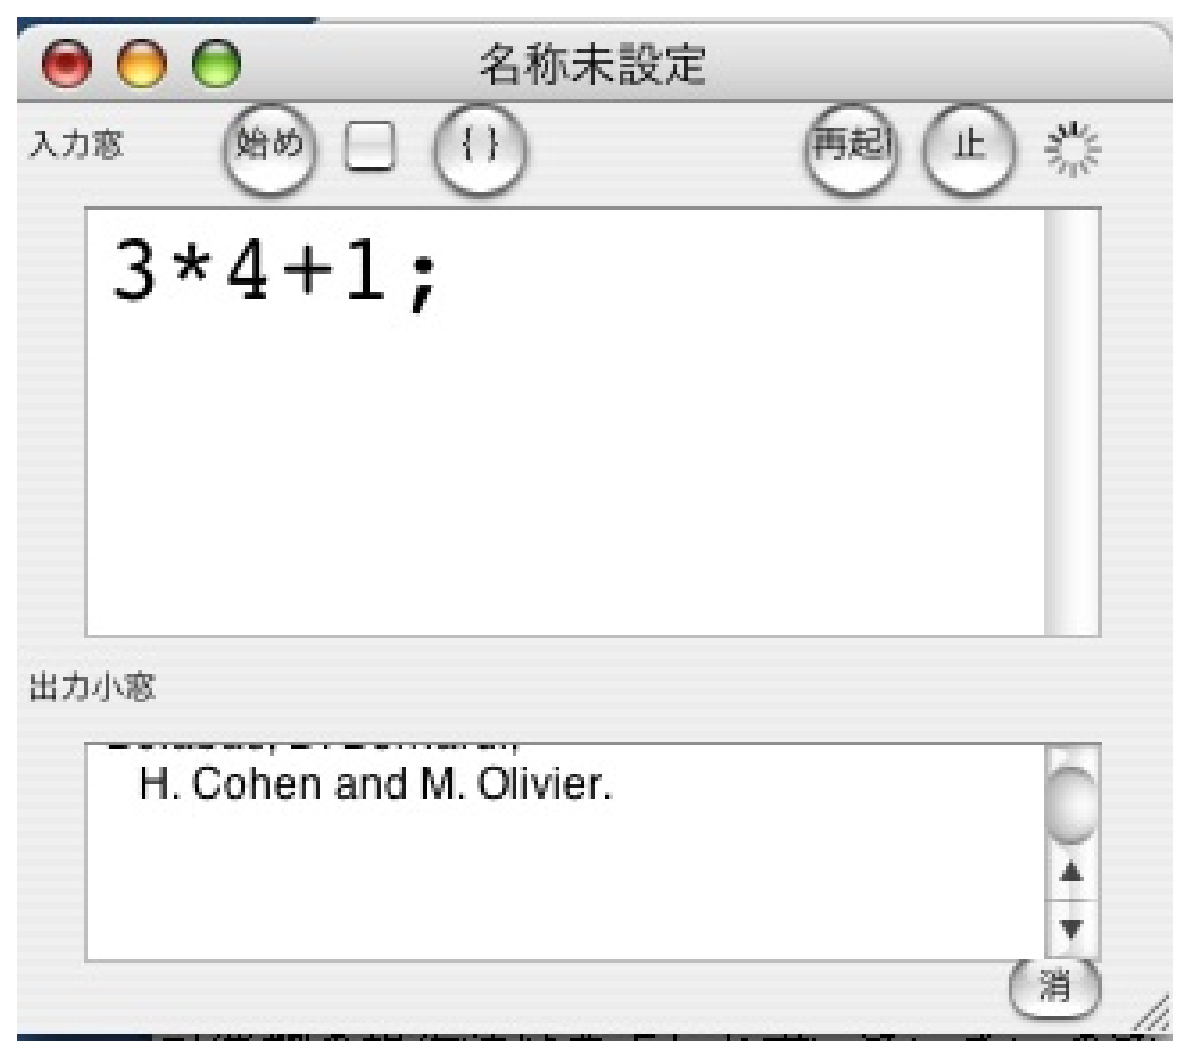
\includegraphics{Figs/cfepStart.ps}}
\caption{ cfep/asir の起動画面} \label{fig:cfepStart}
\end{figure}
%>C

図\ref{fig:cfepStart} の入力窓に計算したい式やプログラムを入力して
``始め''ボタン
%<C
\begin{center}
\scalebox{0.1}{
\includegraphics{Figs/buttonStart.ps}}
\end{center}
%>C
をおすと実行を開始する.
式の計算やプログラムの実行が終了すると,
新しいウインドウ OutputView が開き結果がそのウインドウに表示される.
\index{にゅうりょくまど@入力窓}
\index{OutputView}
``始め''ボタンをおして実行を開始することを計算機用語では 
``入力の評価を始める'' という.
\index{;}  \index{ひょうか@評価}

出力小窓にはシステムからのいろいろな情報が出力されるが,
内容は中上級者向けのものが多い.
\index{しゅつりょくこまど@出力小窓}

ファイルメニュー
%<C
\begin{center}
\scalebox{0.3}{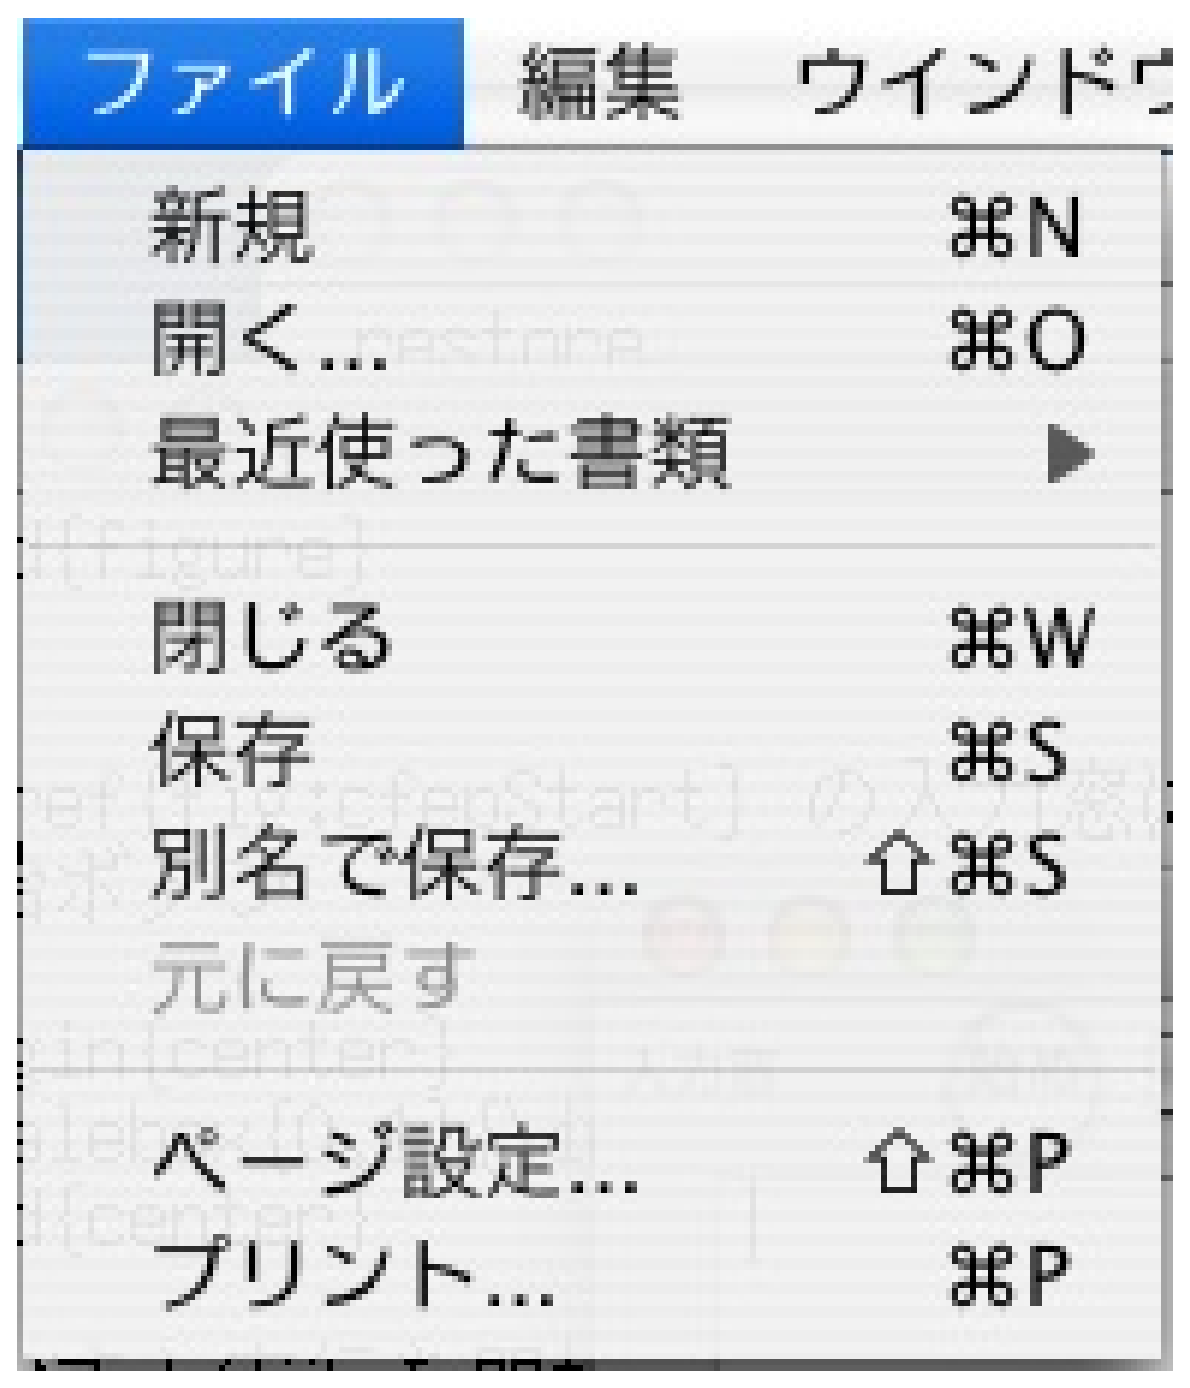
\includegraphics{Figs/menuFile.eps}}
\end{center}
%>C
から''保存''や''別名で保存''を実行すると入力窓の内容をファイルとして保存できる.
出力小窓の内容や OutputView の内容は保存されないので注意してほしい.

cfep/asir を完全に終了するには cfep メニュー
%<C
\begin{center}
\scalebox{0.3}{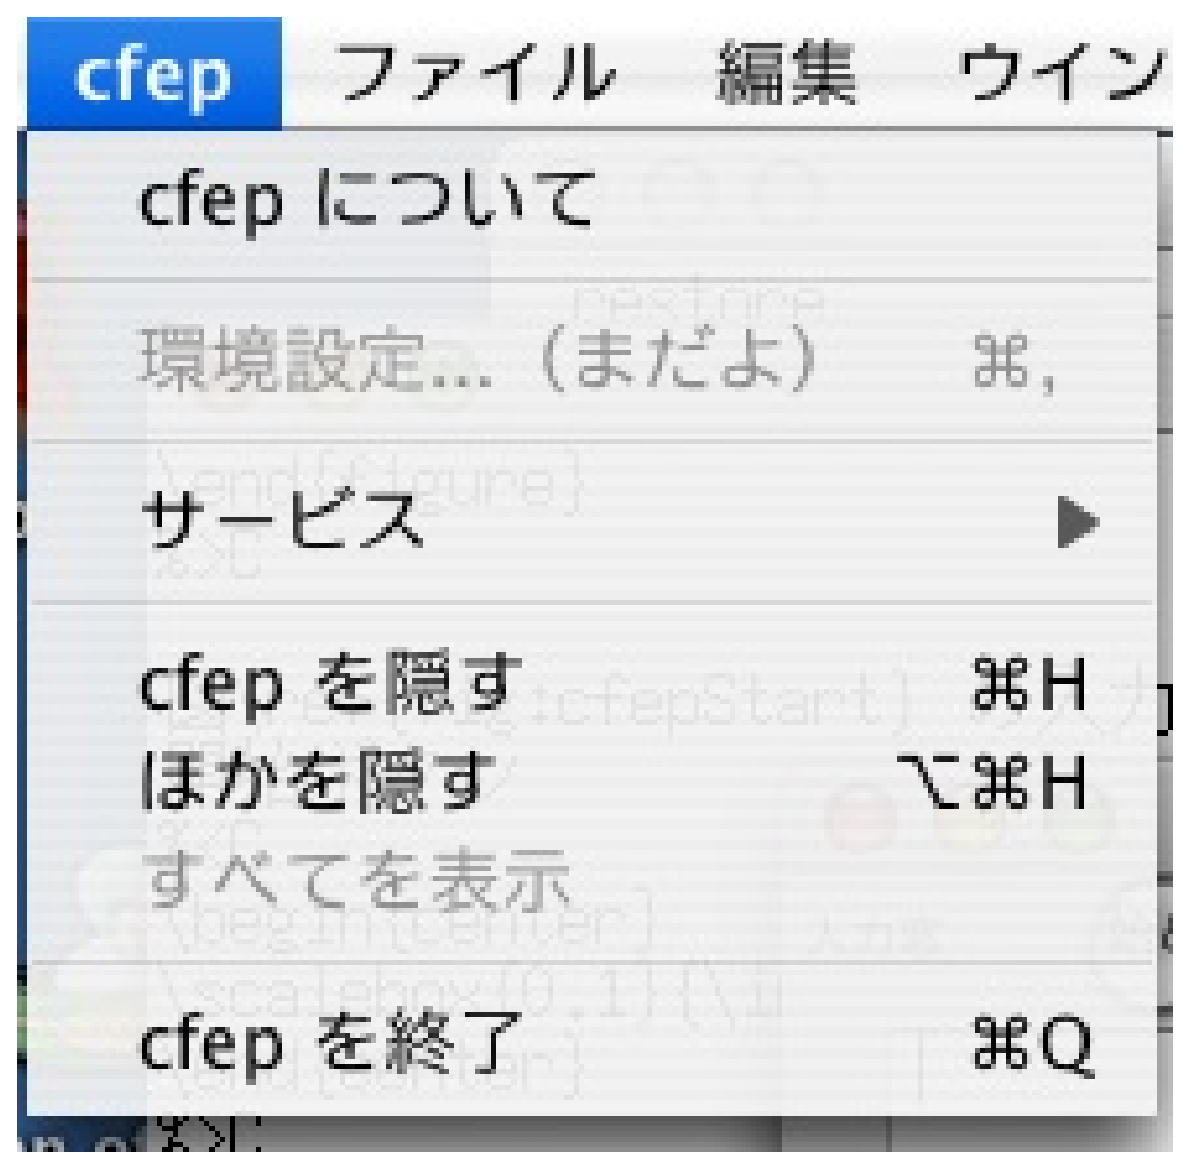
\includegraphics{Figs/menuCfep.eps}}
\end{center}
%>C
の ``cfep を終了'' を実行する.
%en Input \verb@ quit; @ to terminate the Risa/Asir.
%
%

%<C
\bigbreak
\bigbreak

%>C


さて図\ref{fig:cfepStart}では
$ 3 \times 4 + 1 $ の計算をしている.
\begin{screen}
Asir における計算式は普通の数式と似ていて,
足し算は {\tt $+$},
引き算は {\tt $-$}
と書く.
かけ算と割算は $\times$ や ÷ がキーボードにないという歴史的理由もあり,
それぞれ {\tt *} と {\tt /} で表現する.
累乗 $P^N$ は \verb@P^N@ のように \verb@^@ 記号を用いて表す.
\end{screen}

\begin{screen}
式の終りを処理系(asir)に教える(示す)のに {\tt ;} (セミコロン)
を書かないといけない.
文末の ``。'' のような役割を果たす.
またかけ算の記号 {\tt *} の省略はできない. 
\end{screen}

\begin{example} \rm
以下の左の計算式を asir では右のようにあらわす.
\begin{center}
\begin{tabular}{|l|l|} \hline
$2 \times (3+5^4)$  &    \verb@2*(3+5^4);@  \\ \hline
$\left\{\left(2+\frac{2}{3}\right)\times 4+\frac{1}{3}\right\}\times 2 +5  $
                         & \verb@ ((2+2/3)*4+1/3)*2+5; @ \\ \hline
$AX+B$  & \verb@A*X+B;@ \\ \hline
$AX^2+BX+C$ & \verb@A*X^2+B*X+C;@ \\ \hline
$\frac{1}{X-1}$ & \verb@1/(X-1);@ \\ \hline
\end{tabular}
\end{center}
\end{example}

計算の順序は括弧も含めて普通の数式の計算と同じである. 
ただし
数学ではかっことして, {\tt [,]},{\tt \{,\}}などがつかえるが
asir では {\tt (,)} のみ.
{\tt [,]} や {\tt \{,\}}は別の意味をもつ.
上の例のように {\tt (,)} を何重にもつかってよい.
%en In mathematics, {\tt (,)}, {\tt [,]} ,{\tt \{,\}} are used 
%en as brackets in expressions,
%en but in Risa/Asir,  only {\tt (,)} can be used as brackets in expressions,
%en and {\tt [,]} and {\tt \{,\}} are used for different purposes (list and
%en grouping in programs).
この場合括弧の対応関係がわかりにくい.
括弧の対応を調べたい範囲をマウスでドラッグして選択し,
\begin{center}
  \scalebox{0.1}{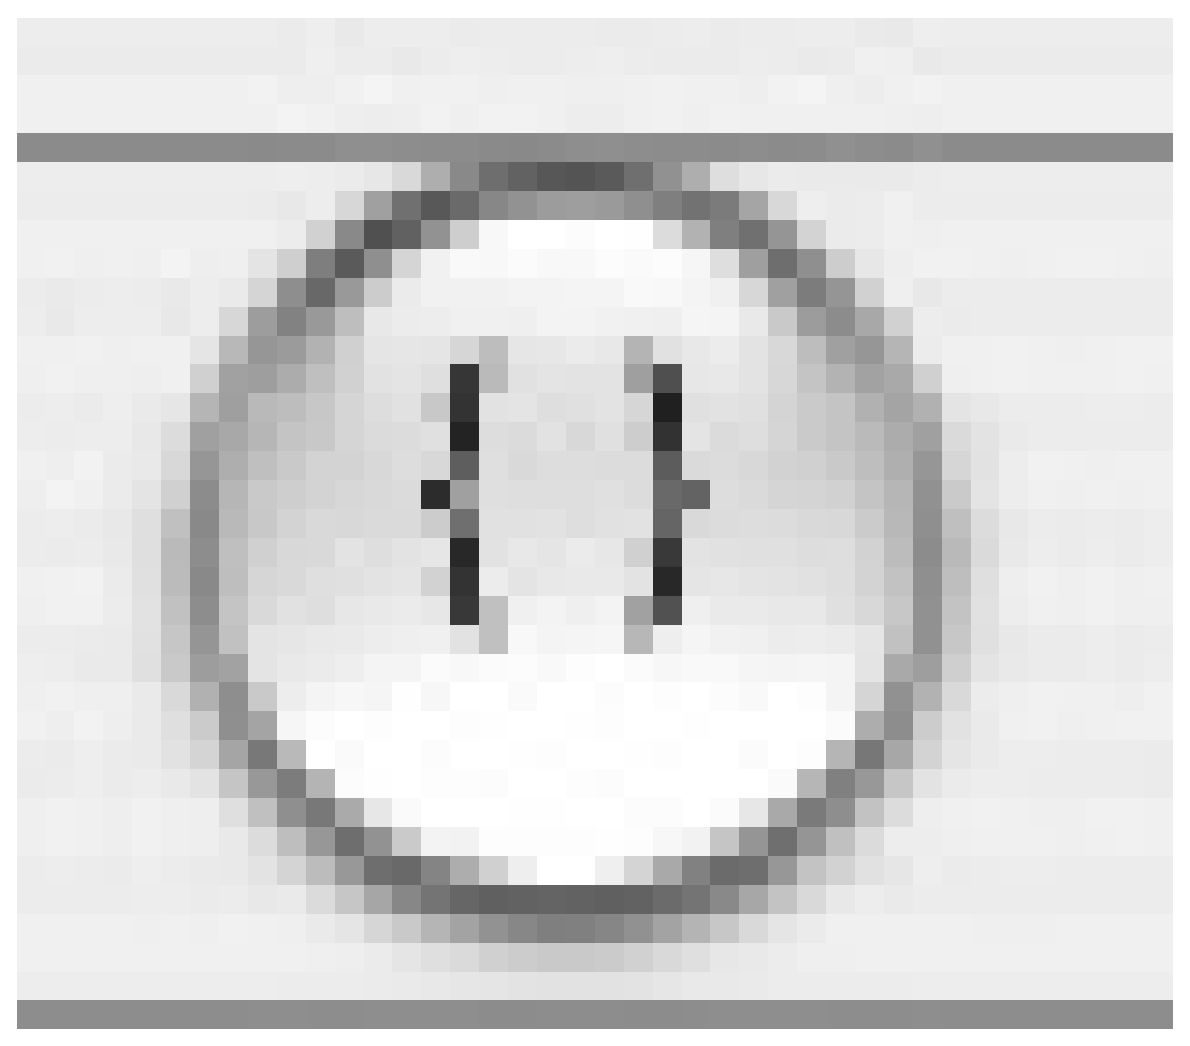
\includegraphics{Figs/buttonBracket.eps}}
\end{center}
ボタンをおすことにより括弧の対応を調べることができる.
\begin{figure}[tb]
\begin{center}
  \scalebox{0.5}{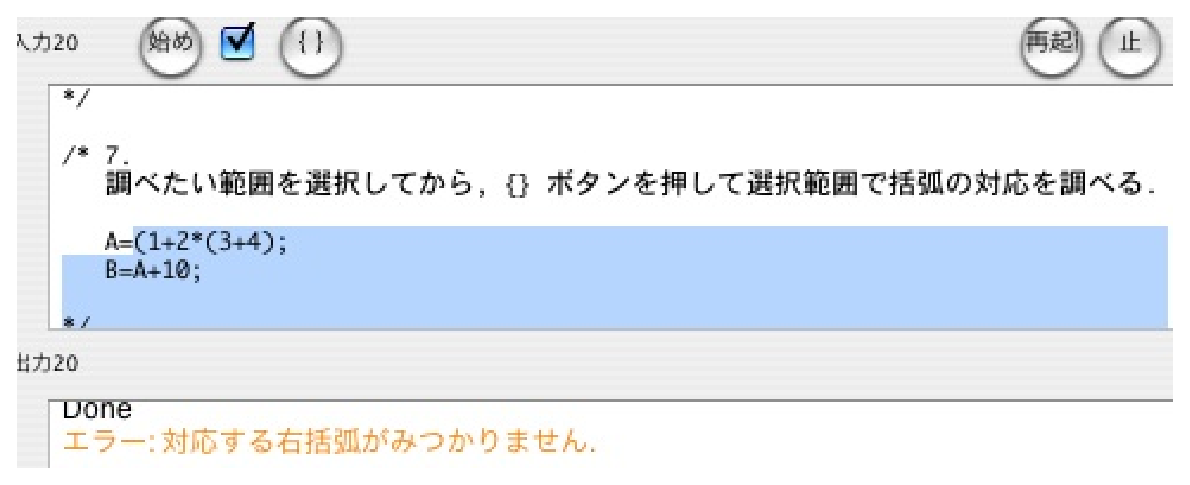
\includegraphics{Figs/menuCheckBracket.eps}}
\end{center}
\caption{括弧の対応} \label{fig:menuCheckBracket}
\end{figure}
図\ref{fig:menuCheckBracket}の例では \verb@(1+2*(3+4))@ と書くべきところを
\verb@(1+2*(3+4)@ と書いておりエラーが表示されている. 

\bigbreak

\noindent \QQQ
``Basic風の使い方を説明する'' と書いてありましたが, Basic って何ですか? \\
\noindent \AAA
コンピュータに仕事をさせるには最終的にはプログラム言語
(計算機への仕事の手順を指示するための人工言語)を用いる.
ワープロ等もプログラム言語で記述されている.
Basic は最も古いプログラム言語の一つであり, 初心者にやさしく, かつ
計算機の仕組みやプログラム言語の理解にも有用である.
Basic は高校の数学の教科書等にも登場する.
著者はいままで ``10進BASIC'' を初心者向け教材として活用していたが, 
``10進BASIC''が MacOS X で動作しないため cfep を開発した.
Asir 言語もプログラム言語であり Basic とよく似ているが, C 言語にもっと近い.


\noindent \QQQ
MacOS X って何ですか? \\
\noindent \AAA
-----まだ書いてない.



%<C
\bigbreak
\noindent
%>C
Asir は数の処理のみならず, $\sqrt{x}$や三角関数の近似計算, 多項式の計算もできる.
%en Asir can do calculations not only for numbers, but also for polynomials.
%en Let us see some examples.
%en 
左の数学的な式は asir では右のように表す.
\begin{center}
\begin{tabular}{|l|l|} \hline
 $\pi$ (円周率) &  {\tt @pi} \\ \hline
 $\cos x$ & {\tt cos(x)} \\ \hline
 $\sin x$ & {\tt sin(x)} \\ \hline
 $\tan x$ & {\tt tan(x)} \\ \hline
 $\sqrt{x}$ & \verb@x^(1/2)@ \\ \hline
\end{tabular}
\end{center}
%en {\tt sin(x), cos(x)} are the trigonometric functions sine and cosine.
%en The symbol {\tt @pi} is the constant $\pi$.
三角関数の角度にあたる部分の $x$ はラジアンという単位を用いて表す.
高校低学年の数学では角度を度(degree)という単位を用いて表すが,
数学3以上では角度はラジアンという単位で表す.
\begin{screen}
90度(直角)が $\pi/2$ ラジアン, 180度が $\pi$ ラジアン.
一般に $d$度は $\frac{d}{180} \pi$ ラジアンである.
\end{screen}
単位ラジアンをもちいると微分法の公式が簡潔になる.
たとえば $x$ がラジアンであると $\sin x$ の微分は $\cos x$ である.
\index{らじあん@ラジアン}

$\sin(x)$ や $\cos(x)$ の近似値を求めるにはたとえば
%en \item  In order to get approximate values of $\sin(x)$  $\cos(x)$, input as
%<C
\begin{center}
\verb@  deval(sin(3.14));  @ 
\end{center}
%>C
と入力する.   
これは $\sin (3.14)$ の近似値を計算する.
$\sin \pi = 0 $ なので $0$ に近い値が出力されるはずである.
実際 {\tt 0.00159265} を出力する.  \index{deval}
{\tt deval}  
(\underline{eval}uate and get a result in {\underline d}ouble number precision の略)
は 64 bitの浮動小数点数により近似値計算する. 
64 bitの浮動小数点数とは何かの説明は超入門の範囲外であるが,
計算機は有限の記憶領域(メモリ)しか持たないので, 小数も有限桁しか扱えない
と覚えておこう. 64bit は扱える桁数を表している.
詳しくは ``asir ドリル'' を参照して欲しい.

%en The function {\tt deval} numerically evaluates the argument in 64 bit floating point arithmetic.
%en As to details, see Chapter \ref{chapter:naibu}.
%en 

\begin{figure}[thb]
\begin{center}
  \scalebox{0.5}{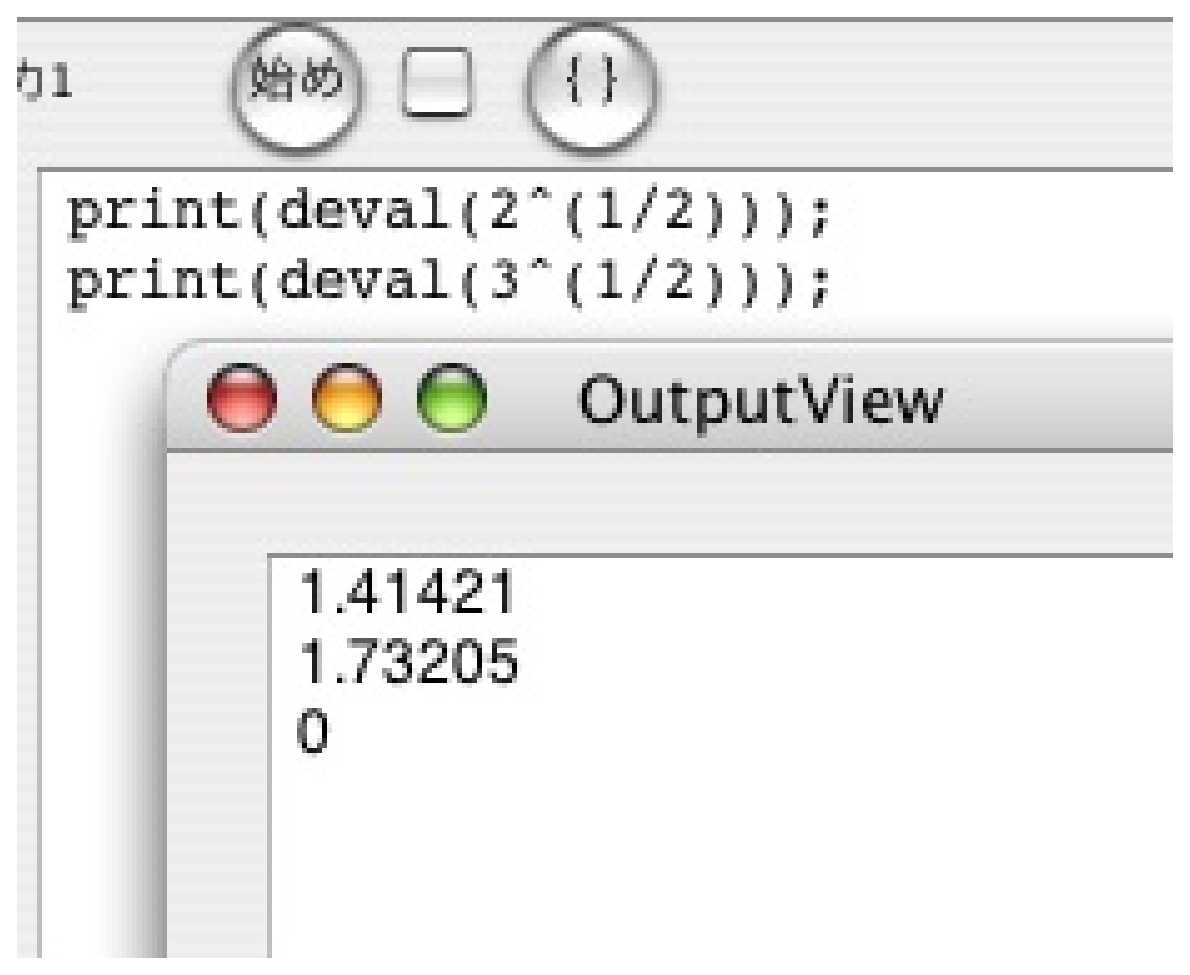
\includegraphics{Figs/sqrt2.eps}} 
\end{center}
\caption{平方根の計算}
\label{fig:sqrt2}
\end{figure}

\begin{example} \rm
$\sqrt{2}$, $\sqrt{3}$ の近似値を計算しなさい. \\
入力
\begin{screen}
\begin{verbatim}
  print(deval(2^(1/2)));
  print(deval(3^(1/2)));
\end{verbatim}
\end{screen}
出力は
図\ref{fig:sqrt2}をみよ.
\end{example}


上の例のように,
セミコロン {\tt ;} で区切られた一連の命令のあつまりはもっとも
単純な asir プログラムの例である.  \index{ぷろぐらむ@プログラム}
一連の命令は始めから順番に実行される.
{\tt print(式等);} は ``式等'' の値を計算して値を画面に表示する.

さて出力の {\tt 1.41421} (ひとよ ひとよに ひとみごろ) は $\sqrt{2}$ の近似値なので,
\verb@print(deval(2^(1/2)));@
の実行結果である. 
さて出力の {\tt 1.73205} (ひとなみに おごれや) は $\sqrt{3}$ の近似値なので,
\verb@print(deval(3^(1/2)));@
の実行結果である. 
最後の {\tt 0} はなんなのであろうか?
実はこれは最後の {\tt print} 文の戻している値である.
むつかしい? 別の例で説明しよう.

\noindent
\fbox{入力}
\begin{screen}
\begin{verbatim}
1+2;
2+3;
3+4;
\end{verbatim}
\end{screen}
この時出力は(OutputViewへの表示は)
\begin{screen}
{\tt 7}
\end{screen}
となる.
cfep/asir ではとくに {\tt print} 文をかかない限り
最後の文の計算結果(評価結果)しか出力しない.
いまの場合は $3+4$  の結果 $7$ を出力している.
\index{しゅつりょくけっか@出力結果}

\begin{problem} \rm
\begin{enumerate}  \index{2のるいじょう@$2$の累乗}
\item $2^8$, $2^9$, $2^{10}$, 
の値を計算して答えを表示するプログラムを書きなさい.
\item $2$ の累乗はパソコンの性能説明によく登場する.
たとえば検索システム google にキーワード ``512 メモリ 搭載'' を入力したところ
``ビデオメモリを 256M から 512M に倍増させ'' など, 数多くの記事がヒットする.
このような記事を(意味がわからなくても)10件あつめてみよう.
$512$ 以外の $2$ の累乗でも同じことを試してみよう.
\item (中級) $2$ の累乗がパソコンの性能説明によく登場する理由を論じなさい.
\end{enumerate}
\end{problem}

\bigbreak

\begin{figure}[thb]
\begin{center}
  \scalebox{0.4}{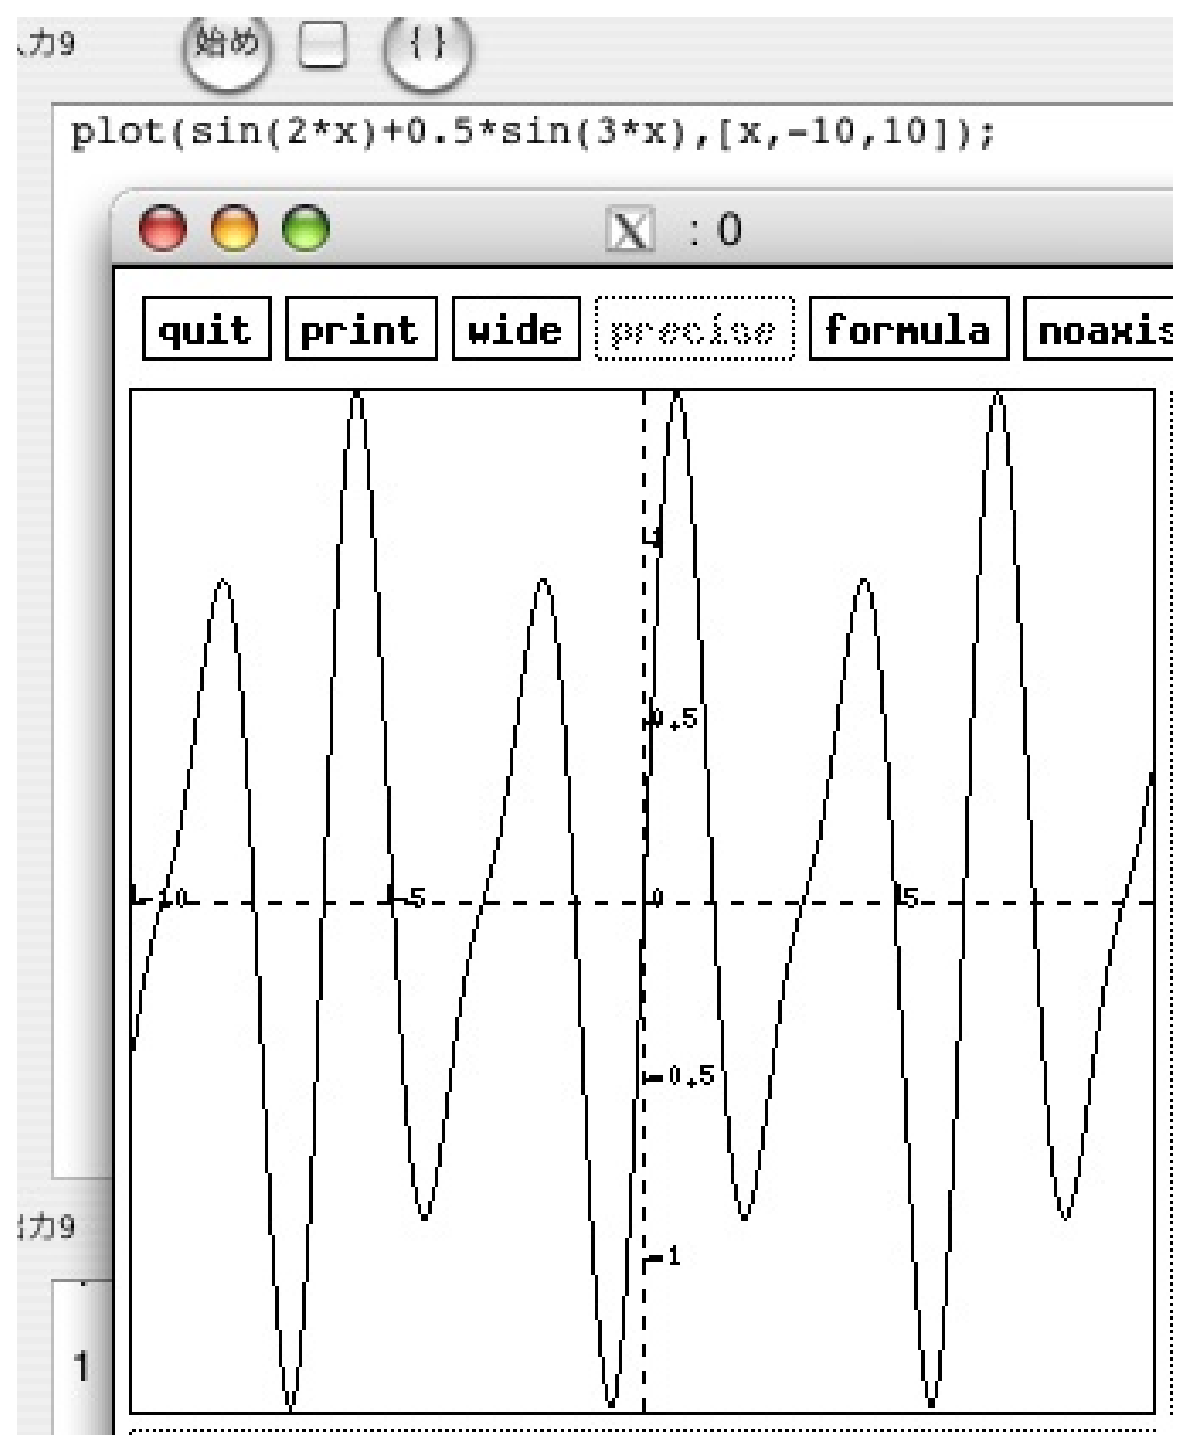
\includegraphics{Figs/plot1.eps}} 
\end{center}
\caption{関数のグラフ}
\end{figure}

\noindent
\HHH
\index{plot}  \index{X11}
%en \begin{example} \rm
%en \index{plot}
\underline{X11 環境が動いていれば},
{\tt plot(f);}   命令で
$x$の関数 $f$ のグラフを描ける.
%en The command {\tt plot(f);}   
%en draws the graph of the function $f$ in the variable $x$.
{\tt x} の範囲を指定したいときはたとえば  \\
{\tt plot(f,[x,0,10])}
と入力すると, {\tt x} は 0 から 10 まで変化する.
%en When you need to specify the range of variables {\tt x}, 
%en input, for example  \\
%en {\tt plot(f,[x,0,10])}
%en Then, the variable {\tt x} runs over $[0, 10]$.

\noindent \fbox{入力例}
%<C
\begin{screen}
\begin{verbatim}
    plot(sin(x));  
    plot(sin(2*x)+0.5*sin(3*x),[x,-10,10]);  
\end{verbatim}
\end{screen}
%>C
\begin{problem} \rm
いろいろな関数のグラフを描いてあそんでみよう.
数学の知識を総動員して計算機の描く形がどうしてそうなのか
説明を試みてみよう.
\end{problem}


\section{エラーメッセージ}

入力にエラーがあると, エラーメッセージが表示される.
\index{えらー@エラー}
\index{えらーめっせーじ@エラーメッセージ}

\begin{figure}[htb]
\begin{center}
  \scalebox{0.5}{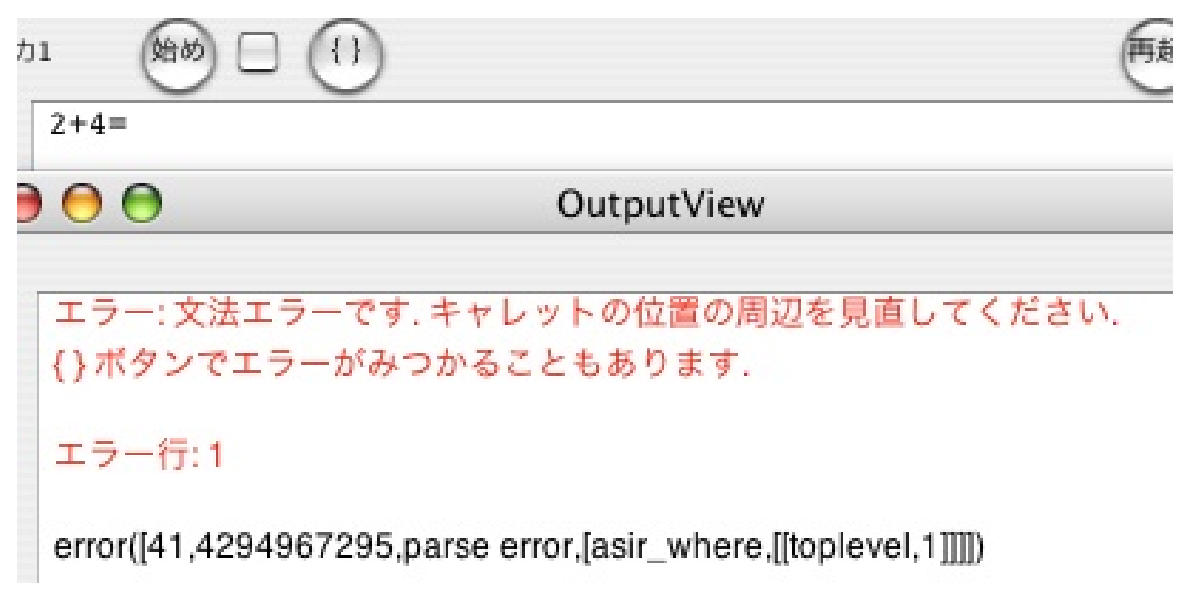
\includegraphics{Figs/errorParseEq}}
\end{center}
\caption{文法エラー} \label{fig:errorParseEq}
\end{figure}
図\ref{fig:errorParseEq} では
\verb@ 2+4= @
と入力している. 最後に \verb@=@ を書く表現は asir の文法では
許されていないので,  ``文法エラー'' と指摘されている.  \index{ぶんぽうえらー@文法エラー}
\begin{screen}
大体これでわかってくれていいじゃない,
とこちらがおもっていてもプログラム言語は一切融通がきかない.
\end{screen}
なお
\begin{verbatim}
error([41,4294967295,parse error,[asir_where,[[toplevel,1]]]])
\end{verbatim}
の部分は上級者向けの情報なのでとりあえず無視してもらいたい.


\begin{figure}[htb]
\begin{center}
  \scalebox{0.5}{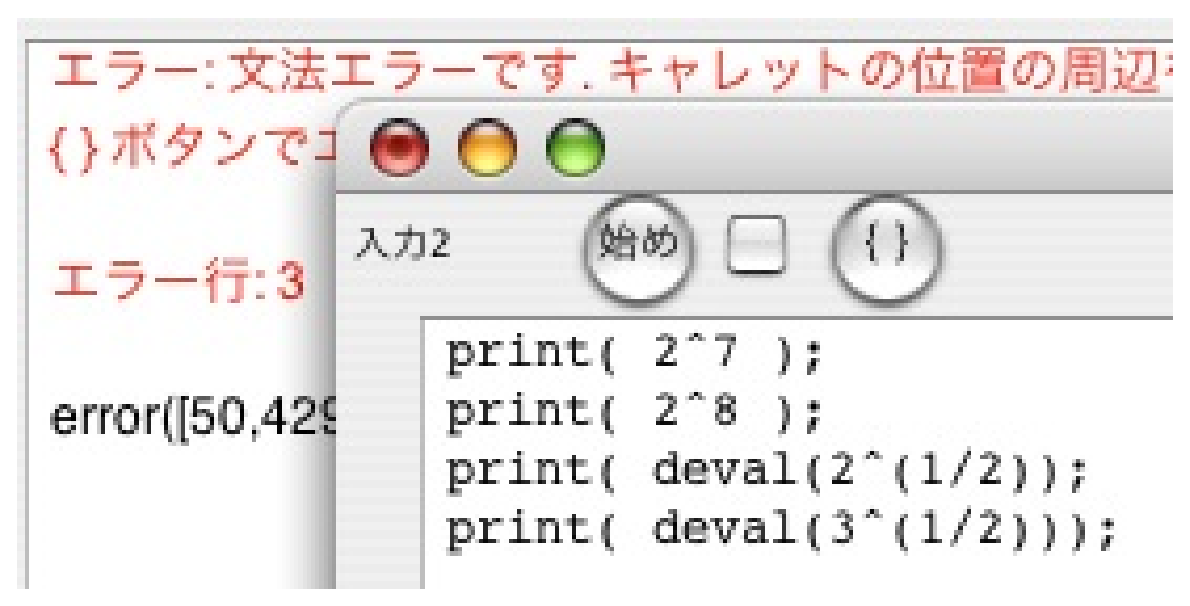
\includegraphics{Figs/errorMultiLine}}
\end{center}
\caption{エラー行} \label{fig:errorMultiLine}
\end{figure}
図\ref{fig:errorMultiLine} では
\begin{screen}
\begin{verbatim}
  print( 2^7 );
  print( 2^8 );
  print( deval(2^(1/2));
  print( deval(3^(1/2)));
\end{verbatim}
\end{screen}
と入力している. 
3行目は右括弧がひとつ足りなくて
\verb@print( deval(2^(1/2)));@
が正しい入力である.
エラー行の3行目にキャレットが自動的に移動しているはずである.
なおプログラムの入力ウインドー内でマウスをクリックすると, せっかく自動移動した
キャレットの位置が変ってしまう. 
プログラムの入力ウインドーのタイトルバーでクリックするとよい.
なおこの例では 
\begin{center}
\scalebox{0.05}{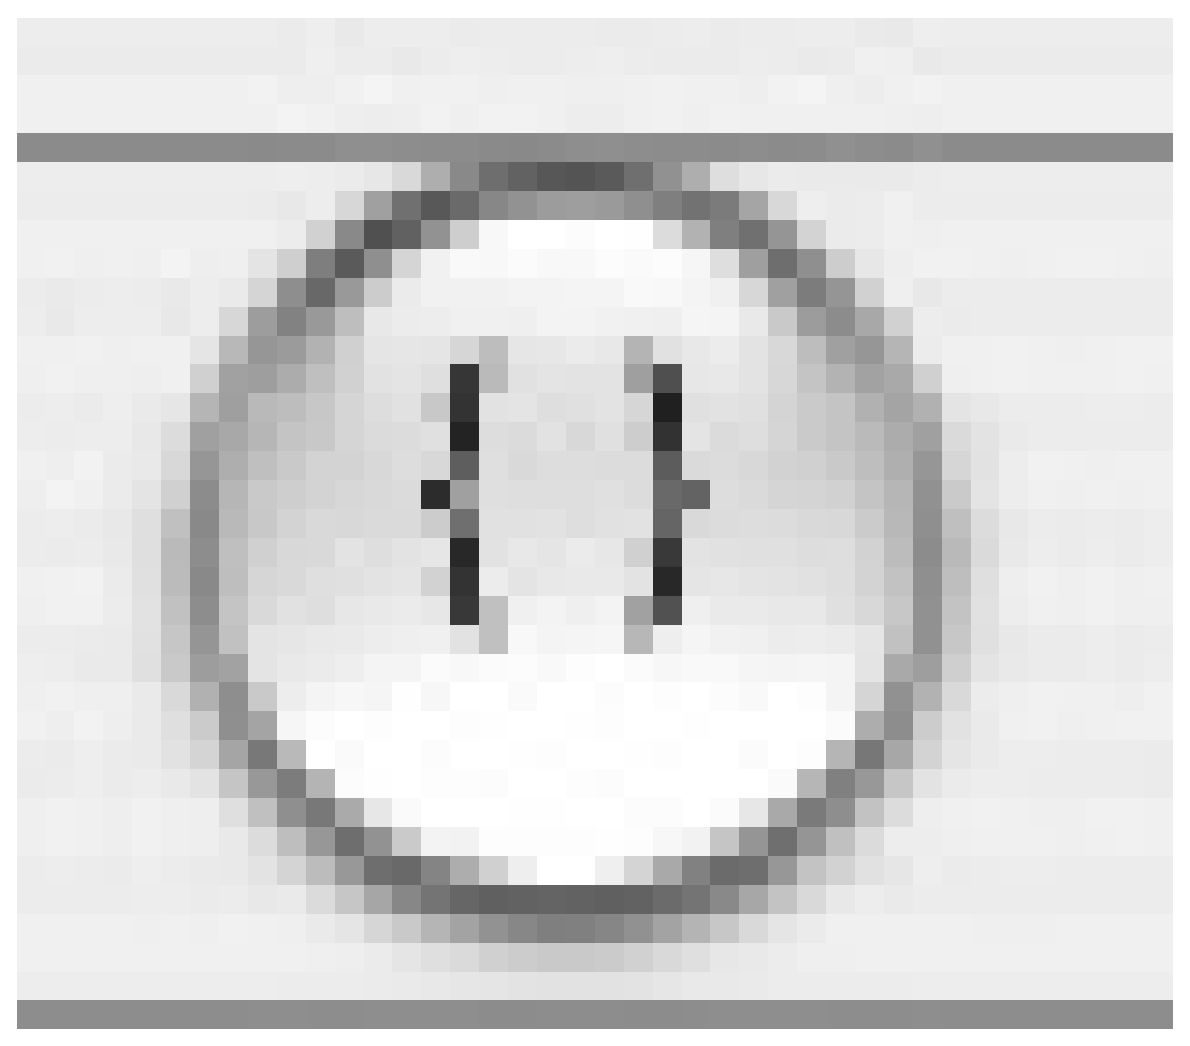
\includegraphics{Figs/buttonBracket.eps}}
\end{center}
ボタンをもちいてもすぐエラーの場所がわかる.
\index{かっこ@括弧}

\noindent {\bf 注意}:
表示された行はエラーの発生位置であるが,
エラーの原因はその前の方の行にあることも多い.
たとえば
\begin{screen}
\begin{verbatim}
1+2
2+3;
\end{verbatim}
\end{screen}
と入力するとエラー行は 2 行目であるが, 原因は1行目で {\tt ; } を 
書き忘れたことである.

\bigbreak
エラー行が複数表示された場合はそれらの中のどこかにエラーがある.
複数あるエラー行に順番にジャンプしていくには,
\fbox{実行} メニューから \fbox{次のエラー行へ} を選択する.
\begin{center}
  \scalebox{0.3}{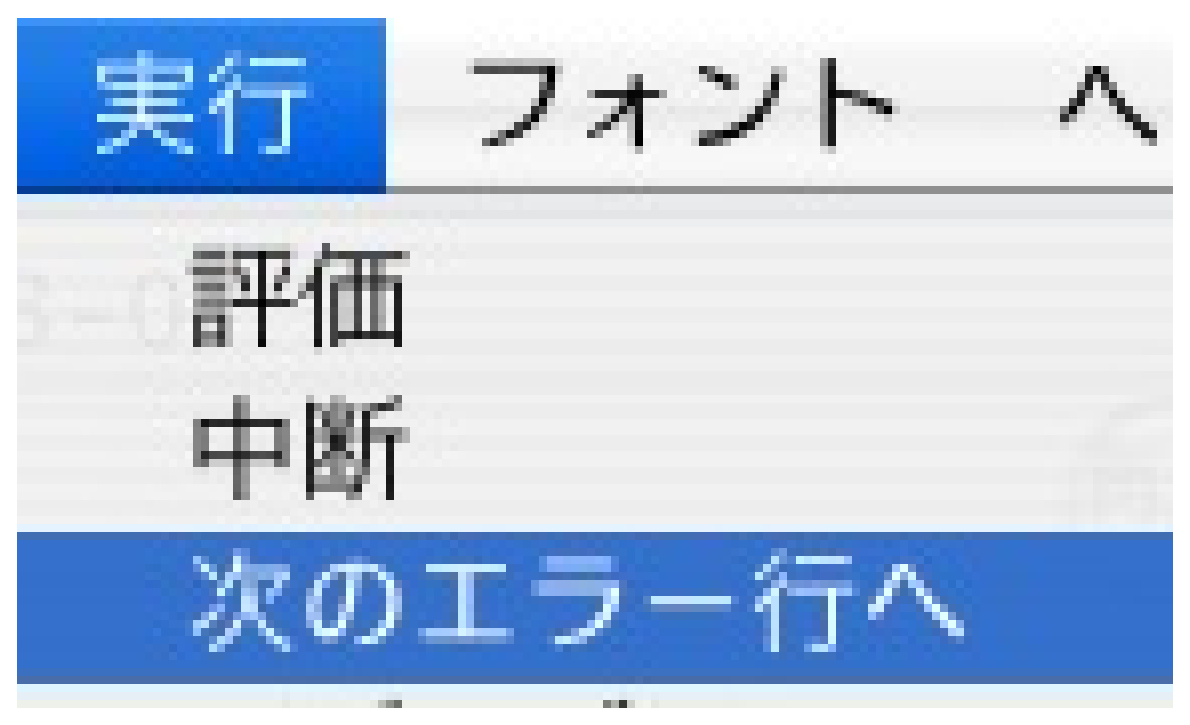
\includegraphics{Figs/menuNextError.eps}}
\end{center}
\index{つぎのえらーぎょうへ@次のエラー行へ}

\begin{problem} \rm
エラーを生じる式またはプログラムを5つ作れ.
\end{problem}


\chapter{ 変数とプログラム }

\section{変数}

\noindent  \index{へんすう@変数}
変数に数値等を記憶しておける.
\underline{変数名は大文字で始まる}.  \index{へんすうめい@変数名}
%英字の大文字, 子文字を区別しているので注意.
なお後述するように asir では多項式計算ができるが小文字で始まる文字列は
多項式の変数名として利用される.   
\index{たこうしきのへんすうめい@多項式の変数名}
%en \noindent
%en Symbols starting with capital alphabetical characters are 
%en {\it program variables}, which are used to store values.
%en \index{program variable}
%en Names of functions defined in programs start with small alphabetical 
%en characters.
%en Note that variable symbols starting with small alphabetical characters are
%en variables in polynomials in Risa/Asir and they cannot be used to store
%en values.
%en 

\index{2のるいじょう@$2$の累乗}
$2$の累乗を表示する次のプログラムを考えよう.
\begin{screen}
\begin{verbatim}
 print( 2^1 );
 print( 2^2 );
 print( 2^3 );
 print( 2^4 );
 print( 2^5 );
 print( 2^6 );
 print( 2^7 );
 print( 2^8 );
\end{verbatim}
\end{screen}
このプログラムは変数 {\tt X} を用いて
次のように書いておけば $2$ の累乗だけなく $3$ の累乗を表示する
のに再利用できる(図\ref{fig:powerOf2}).
\begin{screen}
\begin{verbatim}
  X = 2;
  print( X^1 );
  print( X^2 );
  print( X^3 );
  print( X^4 );
  print( X^5 );
  print( X^6 );
  print( X^7 );
  print( X^8 );
\end{verbatim}
\end{screen}
\begin{figure}[thb]
\begin{center}
\scalebox{0.3}{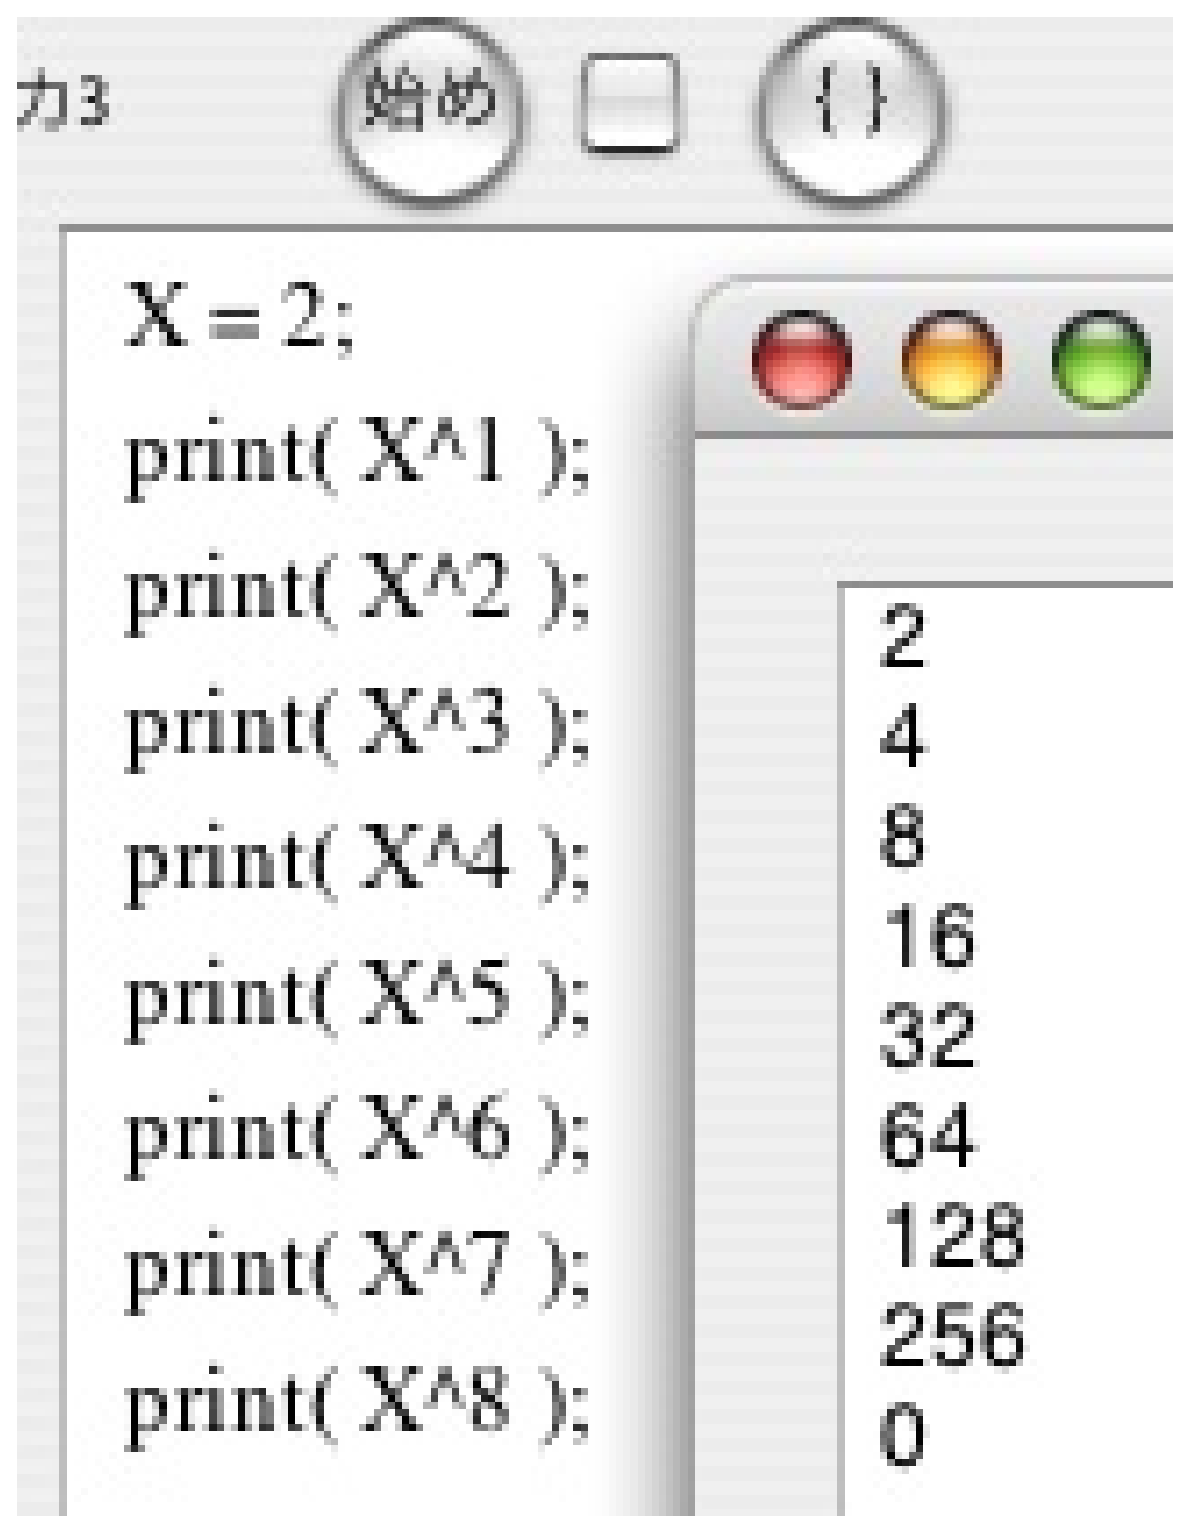
\includegraphics{Figs/powerOf2.eps}}
\end{center}
\caption{変数の利用} \label{fig:powerOf2}
\end{figure}
$3$ の累乗を表示するには
\verb@X=2@ の行を \verb@X=3@ に変更すればいいだけである.

アルファベットの\underline{大文字}ではじまる英数字の列が asir の
変数である.
つまり, {\tt X}, {\tt Y}, {\tt Z} はもちろんのこと,
{\tt Sum} とか {\tt Kazu} とか {\tt X1} など2文字以上の英数字の列
の組み合わせが変数名として許される.


変数を含んだ式をプログラム中で自由につかうこともできる.
たとえば
\begin{verbatim}
  X = 2;
  A = 1;
  print( 2*X^2 -A );
\end{verbatim}
を実行すると {\tt 7} が表示される.

このような例をみると, 変数の機能は
中学数学でならう文字式と似ていると思うだろう.
超入門としてはこれでほぼ正しい理解であるが, よりステップアップしていくには,
次のことを強く記憶しておこう.
\begin{screen}
変数とは計算機に数値等を保存しておくメモリ上の場所の名前である.
\end{screen}

さて, 超入門, 第一の関門である.
\begin{screen}
{\tt =} 記号は次のような形式でつかう:
$$  \mbox{{\bf 変数名}} {\tt = }  \mbox{{\bf 式}} {\tt  ;} $$
これはまず右辺の式を計算しそのあとその計算結果を左辺の変数に代入せよという意味. 
\verb@=@ 記号は右辺を計算してその結果を左辺へ代入せよという\underline{命令}
だと思って欲しい. \\
たとえば,
\verb@X=1@ は \verb@X@ が \verb@1@ に等しいという意味ではなく,
\verb@1@ を 変数 \verb@X@ に代入せよという意味である.
\end{screen}
ここでいいたいことは,  \index{だいにゅう@代入} \index{=} \index{だいにゅうきごう=@代入記号=}
\begin{screen}
\verb@=@ 記号の意味が数学での意味と違うよ!
\end{screen}
ということである.
これで混乱する入門者も多いのでプログラム言語によっては
``$2$ を変数 {\tt X} に代入せよ'' を
\verb@X:=2@ 
と書く場合もある (たとえばプログラム言語 Pascal).

次のプログラムは $2$, $2^2$, $2^4$, $2^8$ を計算して表示する.
\begin{screen}
\begin{verbatim}
  X=2;
  print(X);
  X = X*X;
  print(X);
  X = X*X;
  print(X);
  X = X*X;
  print(X);
\end{verbatim}
\end{screen}
\begin{figure}[thb]
\begin{center}
\scalebox{0.3}{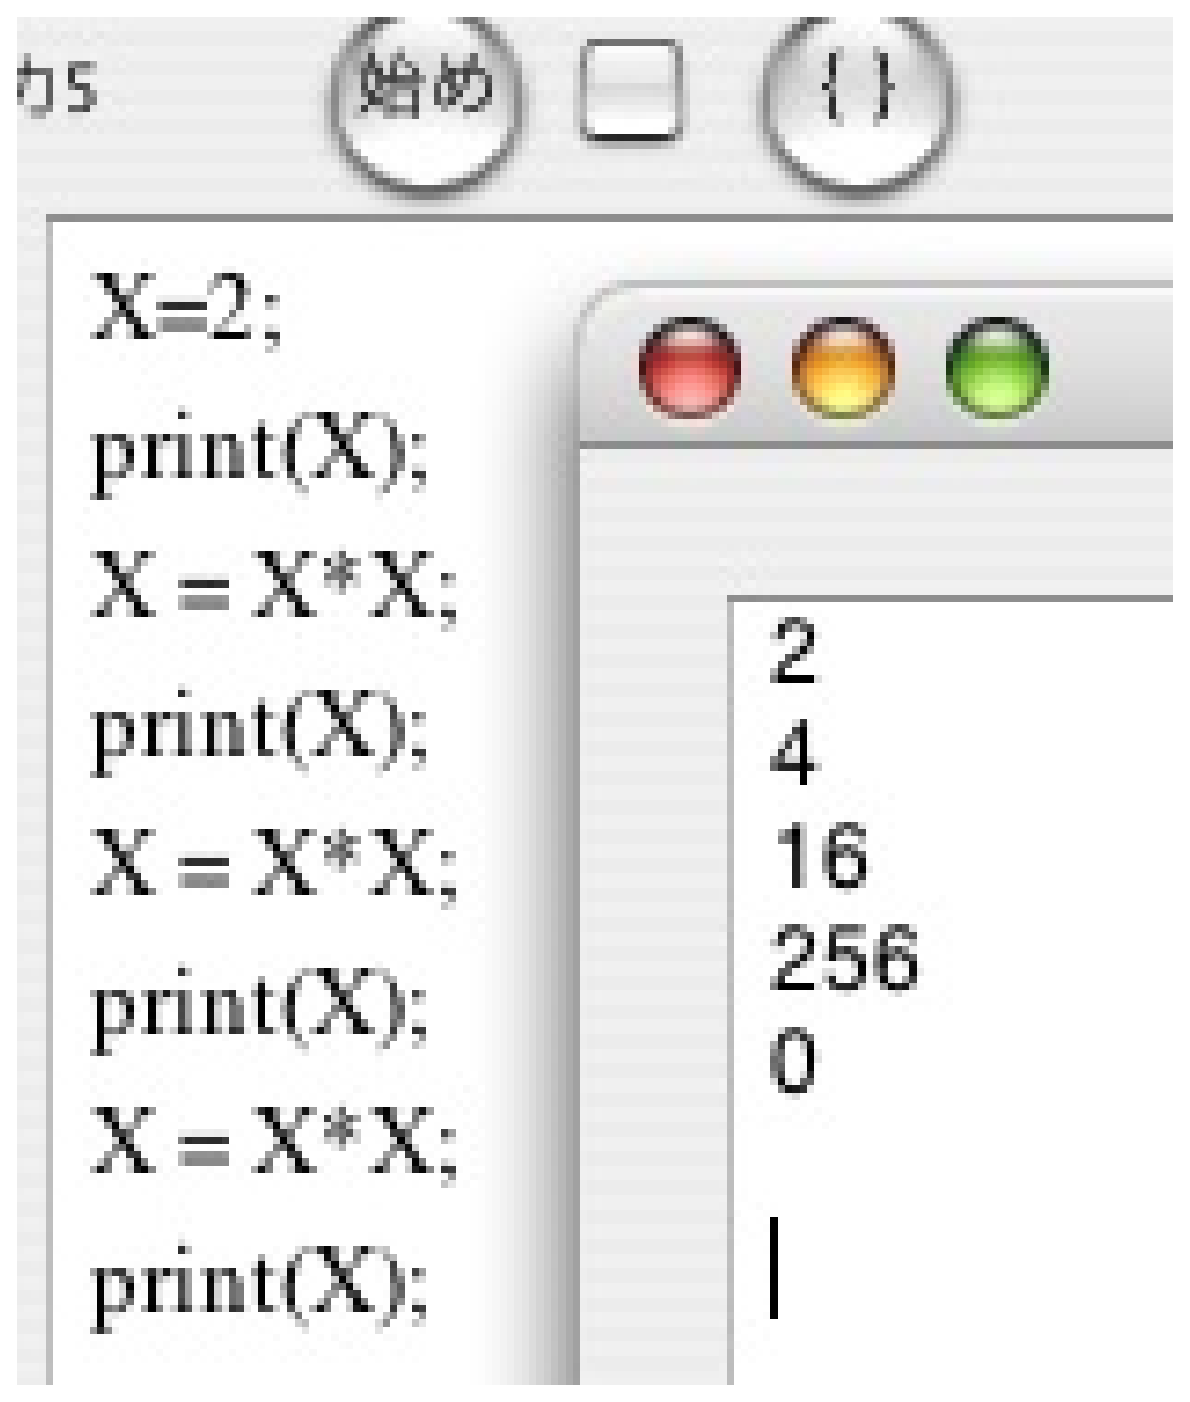
\includegraphics{Figs/powerOf2b.eps}}
\end{center}
\caption{変数の利用} \label{fig:powerOf2b}
\end{figure}
出力が図\ref{fig:powerOf2b}のようになる理由を説明しよう.
まず1行目で変数{\tt X}に2が代入される.
次に3行目ではまず右辺の式を計算する. この場合 {\tt X} の値は $2$ であるので,
$2\times2$ で結果は $4$ である.
\underline{この計算が終った後}結果の $4$ が変数 {\tt X} に代入される.
5行目では右辺の式は $4 \times 4$ なので, その計算結果の $16$ が 左辺の変数 $X$
に代入される.
\index{へんすう@変数}

\bigbreak
%
%
\noindent
\HHH   \index{たこうしき@多項式} \index{すうしきしょり@数式処理}
Asir は多項式計算もできる. 実は Asir は計算機で記号的に数式を処理するための
数式処理システムでもある.
%en Asir can do calculations for polynomials.
\begin{enumerate}
%en \begin{enumerate}
\item 小文字ではじまる記号は多項式の変数である.
数学とちがって変数の名前は一文字とはかぎらない.
たとえば {\tt rate} と書くと,  $rate$ という名前の多項式の変数となる.
たとえば {\tt x2} と書くと,  $x2$ という名前の多項式の変数となる.
$x$ かける $2$ は {\tt x*2} と書く.  \index{たこうしきへんすう@多項式変数}
%en \item Symbols starting small alphabetical character are variables of polynomials. For example, {\tt x2} is the variable of the name x2.
%en The expression {\tt x*2} stands for $x$ times $2$.
%
%
\item   \index{いんすうぶんかい@因数分解}  \index{fctr}
{\tt fctr(\poly)} は \poly を有理数係数の範囲で因数分解する.
{\tt fctr} は factor の短縮表現である. 
%en \item   \index{factorization}  \index{fctr}
%en The input {\tt fctr(\poly)} factors \poly in the ring of polynomials
%en with rational number coefficients.
%
% 
\end{enumerate}
%en \end{enumerate}

\begin{figure}[tbh]
\begin{center}
\scalebox{0.3}{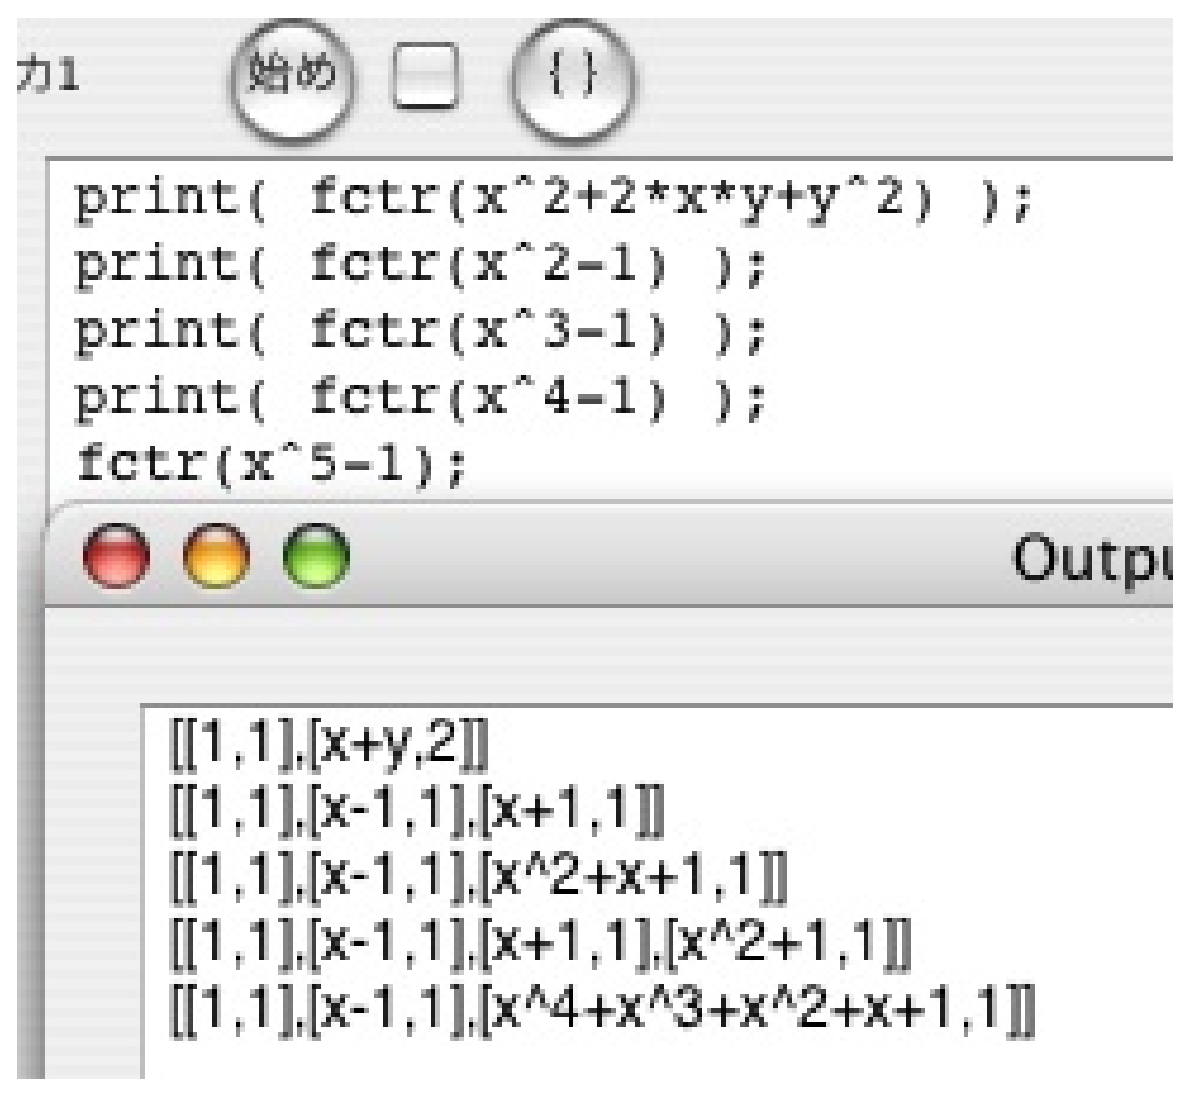
\includegraphics{Figs/fctr1.eps}}
\end{center}
\caption{因数分解} \label{fig:fctr1}
\end{figure}

図\ref{fig:fctr1} の{\tt fctr} の出力の最初は $x^2+2xy+y^2$ が 
$ 1^1 \times (x+y)^2 $ 
と因数分解されることを意味している. 
図\ref{fig:fctr1} の{\tt fctr} の出力の2番目は $x^2-1$ が 
$$ 1^1 \times (x-1)^1 \times (x+1)^1 
$$ 
と因数分解されることを意味している. 


\section{くりかえし}

くりかえしや判断をおこなうための文が asir には用意されている.
この文をもちいると複雑なことを実行できる.
まず一番の基礎であるくりかえしの機能をためしてみよう.
\index{くりかえし} \index{forぶん@for文}
%en A programming language is installed in Asir. 
%en Let us try the most basic programming; repeating and printing.
\begin{example} \rm
図\ref{fig:powerOf2}のプログラムは次のように繰り返し機能 --- {\tt for}文 ---
を用いて簡潔に書ける.
\begin{screen}
\begin{verbatim}
  X = 2;
  for (I=1; I<=8; I++) {
     print( X^I );
  }
\end{verbatim}
\end{screen}
実行結果は図\ref{fig:powerOf2For}をみよ.
\end{example}

\begin{figure}[tbh]
\begin{center}
\scalebox{0.3}{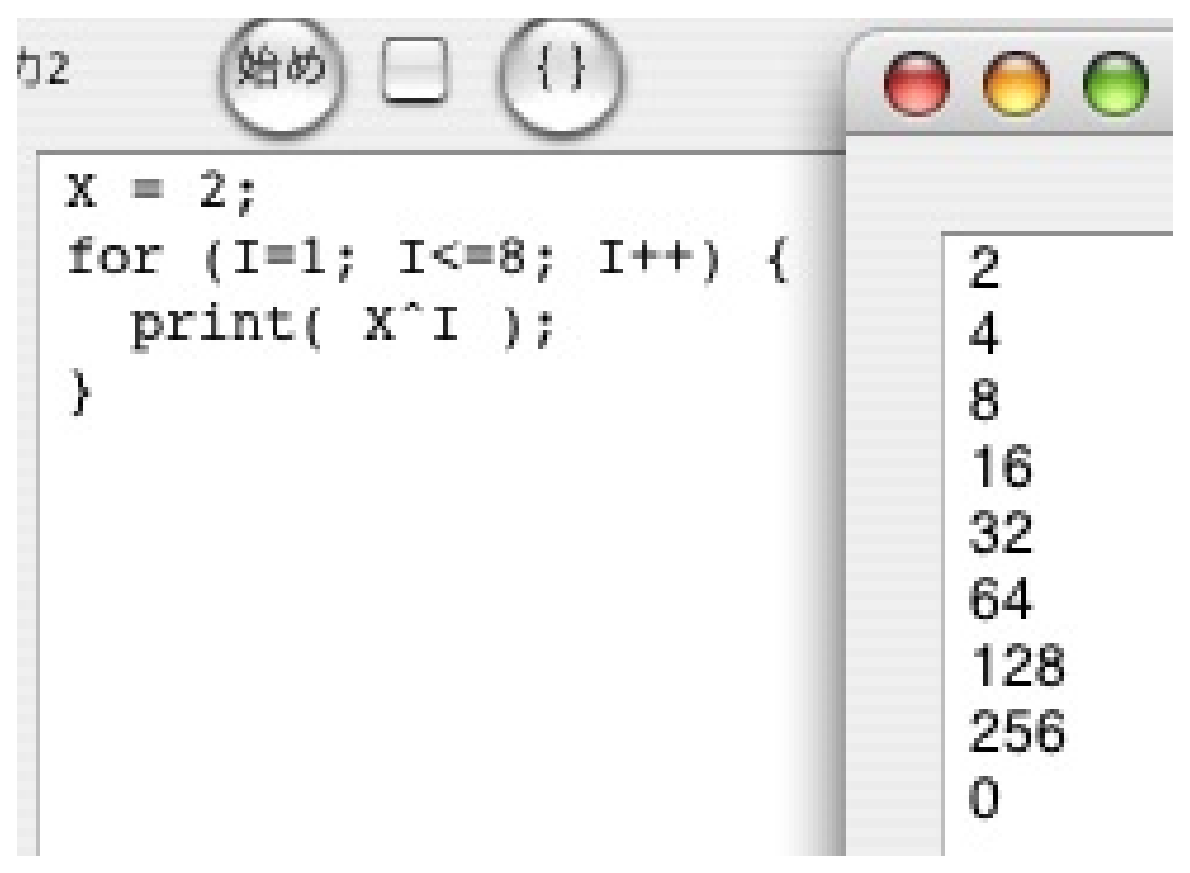
\includegraphics{Figs/powerOf2For.eps}}
\end{center}
\caption{for文} \label{fig:powerOf2For}
\end{figure}


繰り返し関連の表現の意味を箇条書にしてまとめておこう.
\begin{enumerate}
%en \begin{enumerate}
\item   \index{for} \index{くりかえし@繰り返し} \index{\<@\verb&<=&}
%en \item   \index{for} \index{repeat} \index{\<@\verb&<=&}
\verb@ for (K=初期値; K<=終りの値; K++) {ループの中で実行するコマンド}; @
はあることを何度も繰り返したい時に用いる.
for ループと呼ばれる.
``{\tt K<=N}'' は, ``${\tt K} \leq {\tt N}$か'' という意味である.
似た表現に,
``{\tt K>=N}''があるが, これは ``${\tt K} \geq {\tt N}$か'' という意味である.
{\tt =} のない
``{\tt K<N}'' は, ``${\tt K} < {\tt N}$か'' という意味である.
\item \verb@ ++K @ や \verb@ K++ @ は {\tt K} を 1 増やせという意味である.
\verb@ K = K+1 @ と書いてもよい.
同じく, \verb@ --K @ や \verb@ K-- @ は {\tt K} を 1 減らせという意味である.
%en The sentence 
%en {\tt for (K={\it initial value}; K<={\it limit}; K++) \{{\it commands}\}; }
%en is used to repeat commands.
%en It is called the ``for'' loop.
%en ``{\tt K<=N}'' means that ``${\tt K} \leq {\tt N}$ holds''. 
%en A similar expression
%en ``{\tt K>=N}'' implies that ``${\tt K} \geq {\tt N}$ holds''
%en The expression ``{\tt K<N}'' means that ``${\tt K} < {\tt N}$''.
%en \item The expressions \verb@ ++K @ and \verb@ K++ @ mean increasing 
%en {\tt K} by $1$.
%en In this example, it has the same meaning with \verb@ K = K+1 @.
%en Similarly \verb@ --K @ and \verb@ K-- @ mean decreasing {\tt K} by 1.
%
%
\end{enumerate}
%en \end{enumerate}
%en

\begin{figure}[tbh]
\begin{center}
\scalebox{0.3}{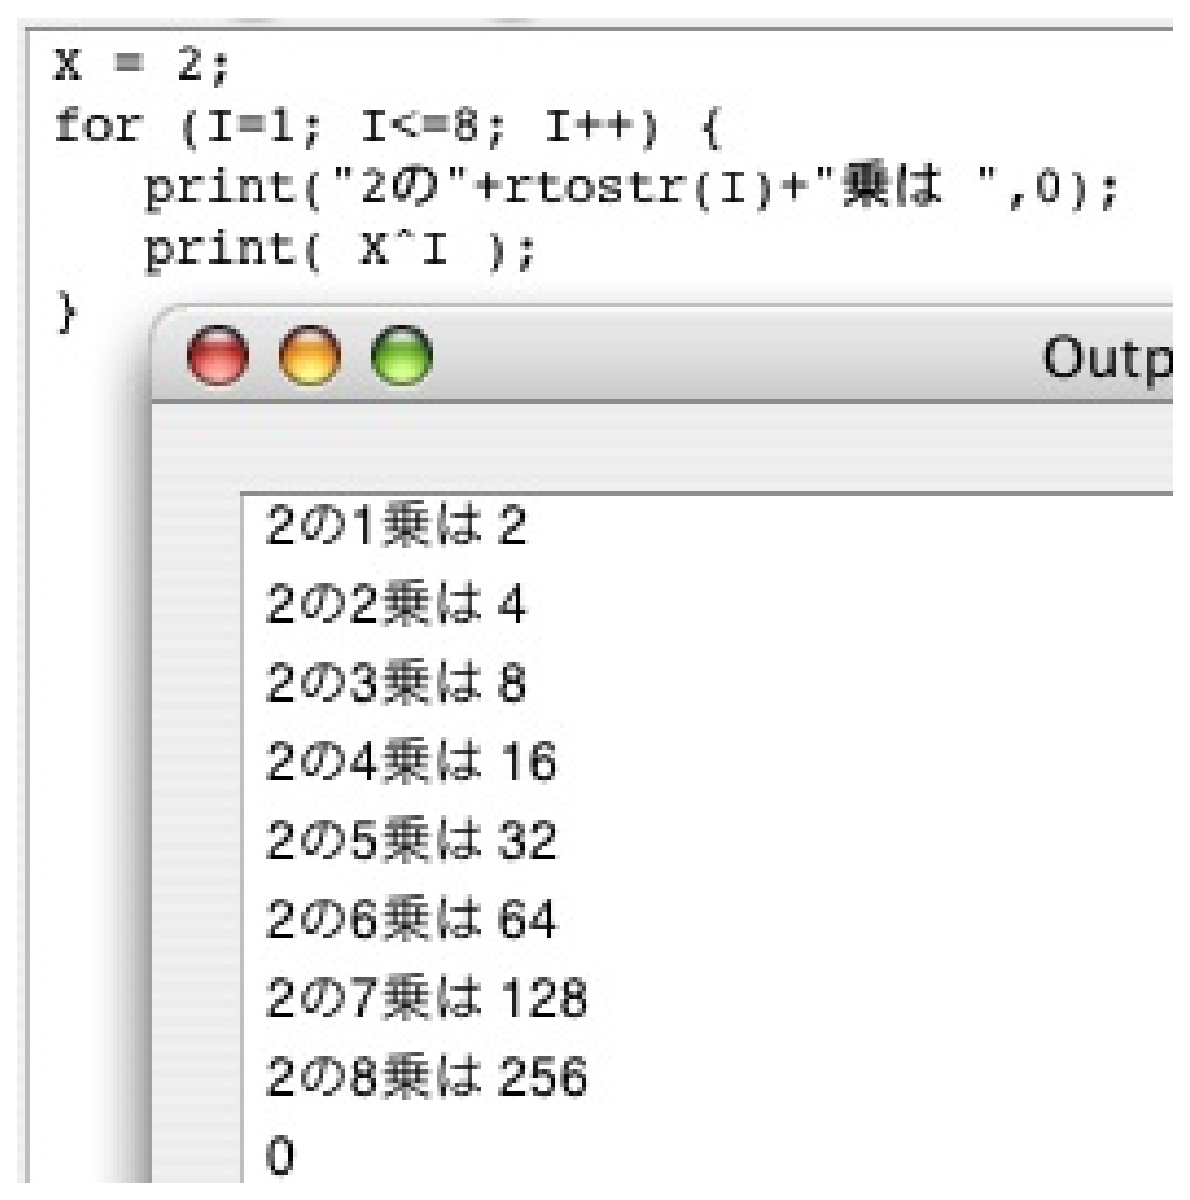
\includegraphics{Figs/powerOf2For2.eps}}
\end{center}
\caption{for文} \label{fig:powerOf2For2}
\end{figure}
for のあとの {\tt \{}, {\tt \}} の中には複数の文(命令)を書ける.
\begin{screen}
\begin{verbatim}
  X = 2;
  for (I=1; I<=8; I++) {
     print("2の"+rtostr(I)+"乗は ",0);
     print( X^I );
  }
\end{verbatim}
\end{screen}
この例では  
日本語を含むので前の節で述べたように日本語空白をプログラム本体にいれないようにして,
注意深くプログラムを入力してもらいたい.  
実行結果は図\ref{fig:powerOf2For2}をみよ. \index{2のるいじょう@$2$の累乗}
\verb@print("2の"+rtostr(I)+"乗は ",0);@ の部分を簡単に説明しておこう.
まず最後の {\tt 0} は出力のあと改行しない, つまり次の {\tt print} 文の出力を
そのまま続けよという意味.   \index{print} \index{rtostr}
\verb@"@ でかこまれた部分は文字列と呼ばれている.これはこのまま表示される.
\verb@rtostr(I)@ は数字 {\tt I} を文字列表現に変換しなさい, という意味
(超入門としては難しい?).
あと文字列に対して {\tt +} を適用すると文字列が結合される.
\index{もじれつのけつごう@文字列の結合}
\index{もじれつひょうげん@文字列表現}


\noindent
\fbox{雑談}
(江戸時代の数学の本にあった問題の改題) \\
殿様: このたびの働きはあっぱれであった. 褒美はなにがよいか? \\
家来: 今日は一円, 明日は2円, 明後日は4円と, 前日の2倍づつ, これを4週間続けて
くださるだけで結構でございます. \\
殿様: なんともささやかな褒美じゃのう. よしよし. \\
さて, 家来はいくら褒賞金をもらえるだろう?
これもまた$2$の累乗の計算である. \index{2のるいじょう@$2$の累乗}
Cfep/asir で計算してみよう.



\begin{example}\Begin \quad
{\tt for} による繰り返しを用いて $\sqrt{x}$ の数表をつくろう.
%en \begin{example}\Begin [02] \quad
%en By using {\tt for} loop, generate a table of  $\sqrt{x}$.
%en \end{example}
%en 
\begin{screen}
\begin{center}
\begin{verbatim}
  for (I=0; I<2; I = I+0.2) {
     print(I,0); print(" : ",0);
     print(deval(I^(1/2)));
  }
\end{verbatim}
\end{center}
\end{screen}
%>C
出力結果
%en Output.
%<C
\begin{center}
\begin{tabular}{|l|} \hline \sl
0 : 0 \\
0.2 : 0.447214 \\
0.4 : 0.632456 \\
0.6 : 0.774597 \\
0.8 : 0.894427 \\
1 : 1 \\
1.2 : 1.09545 \\
1.4 : 1.18322 \\
1.6 : 1.26491 \\
1.8 : 1.34164 \\
2 : 1.41421 \\
\hline 
\end{tabular}
\end{center}
%>C
\rm
\index{print}
{\tt print(A)} は変数 {\tt A} の値を画面に表示する.
{\tt print(文字列)} は文字列を画面に表示する.
{\tt print(A,0)} は変数 {\tt A} の値を画面に表示するが, 表示した
あとの改行をしない.
空白も文字である.したがって, たとえば
{\tt A=10; print(A,0); print(A+1);} 
を実行すると,   \index{print}
{\tt 1011} と表示されてしまう.
{\tt A=10; print(A,0); print(" ",0);print(A+1);} 
を実行すると,
{\tt 10 11} と表示される.
%en \rm
%en \index{print}
%en The command {\tt print(A)} displays the value of the variable {\tt A}
%en on the screen.
%en The command {\tt print({\it string})} outpus the {\it string} on the screen.
%en The command {\tt print(A,0)} displays the value of the variable {\tt A},
%en but it does not make the newline.
%en Note that the blank is a character. For example, if you input
%en {\tt A=10; print(A,0); print(A+1);} 
%en {\tt 1011} will be displayed.   So, input as 
%en {\tt A=10; print(A,0); print(" ",0);print(A+1);} 
%en Then,
%en {\tt 10 11} will be displayed.
%en 
\end{example}

ところで, この例では条件が ${\tt I}<2$ なのに ${\tt I}=2$ 
の場合が表示されている.
実際に asir 上で実行してみるとこうなるが, 理由を知るには、
浮動小数の計算機上での表現についての知識が必要である
(``asirドリル''を参照).
とりあえず, 
%en In this example, the termination condition is ${\tt I}<2$, but
%en the case of ${\tt I}=2$ is executed. In order to understand the reason,
%en we need to study the format of floating point numbers.
%en (See \ref{chapter:naibu} for details).
%en For now, please keep the following in our mind.
\begin{FRAME}
整数や分数の計算は Asir 上で正確に実行されるが,
小数についてはそうでない. 
\end{FRAME}
と覚えておこう.
%en \begin{FRAME}
%en Arithmetics for integers and rational numbers are exact in Risa/Asir,
%en but arithmetics for dicimal numbers are not.
%en \end{FRAME}
%en 

\begin{problem}
  あたえられた 10 進数を 2進数へ変換するプログラムを作れ.
 ヒント: {\tt A}÷{\tt B} の余りは \verb@A%B@ で計算できる.
  \index{あまり@余り}
\end{problem}

\section{実行の中止}
%
%
\index{ちゅうし@中止}  \index{interrupt}
実行中の計算やプログラムの実行を中止したい時は中止ボタン
\begin{center}
\scalebox{0.1}{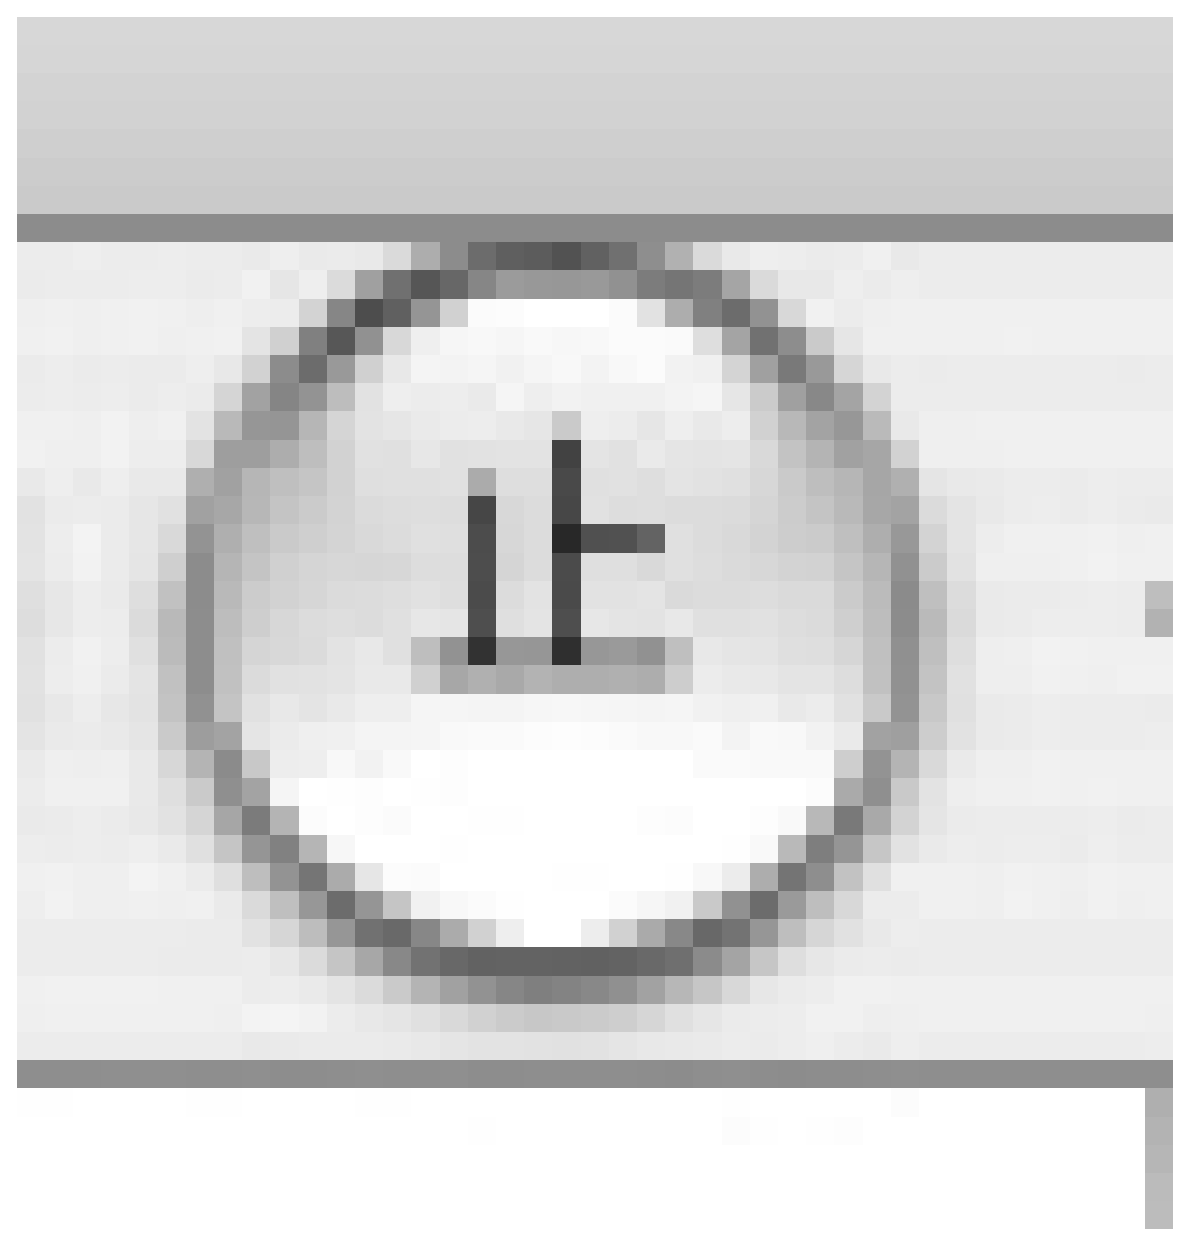
\includegraphics{Figs/buttonStop.eps}}
\end{center}
をクリックする.

\begin{figure}[tbh]
\begin{center}
\scalebox{0.5}{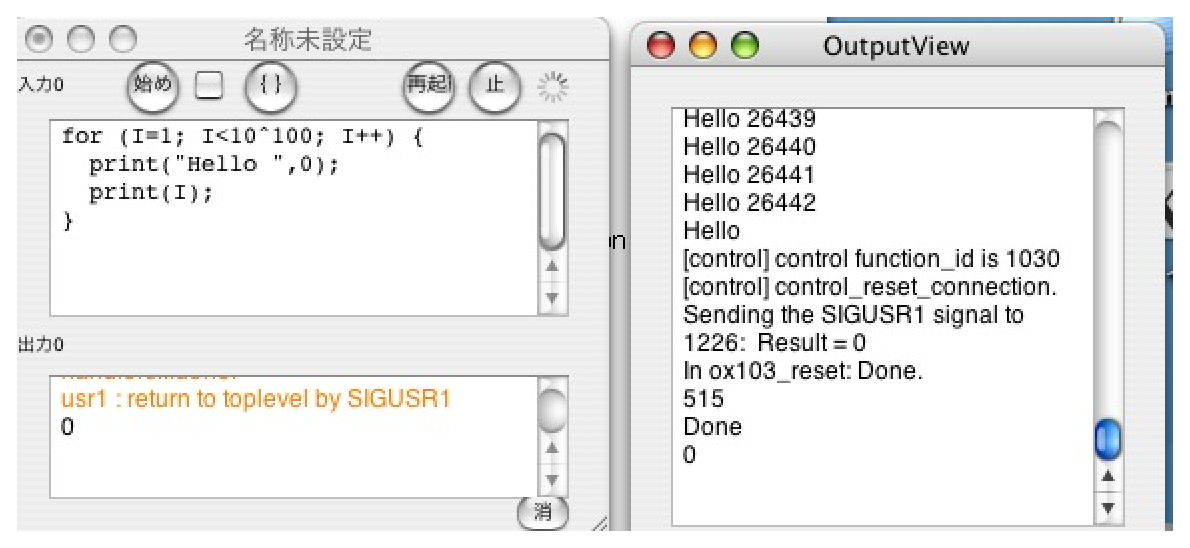
\includegraphics{Figs/interrupt.eps}}
\end{center}
\caption{実行の中止} \label{fig:interrupt}
\end{figure}

図\ref{fig:interrupt}では
$10^{100}$ 回の {\tt Hello } の出力の繰り返しを中止している.

cfep は開発途上のシステムのため
\begin{verbatim}
[control] control function_id is 1030
[control] control_reset_connection.
Sending the SIGUSR1 signal to 1226:  Result = 0
In ox103_reset: Done.
515
Done
\end{verbatim}
このような開発者専用のメッセージも出力されるが,
とりあえずこのようなメッセージがでたら中止が成功したということである.


\section{エンジン再起動}

\index{さいきどう@再起動}  \index{けいさんえんじん@計算エンジン}
\index{けいさんさーば@計算サーバ}
Cfep/asir では次のように3つのプロセスが互いに通信しながら動作している.
\begin{center}
\fbox{cfep} $\Leftrightarrow$ \fbox{コントローラ(ox\_texmacs)}
$\Leftrightarrow$ \fbox{計算エンジン(ox\_asir)}
\end{center}
計算エンジン(計算サーバ)を再起動したり別のものにとりかえたりできる.
\index{けいさんえんじん@計算エンジン}
\index{けいさんさーば@計算サーバ}
\index{えんじん@エンジン}

\index{さいきどう@再起動}  \index{restart}
エンジン再起動ボタン
\begin{center}
\scalebox{0.05}{
\includegraphics{Figs/buttonRestart}}
\end{center}
をクリックすると,
現在利用している計算エンジンを停止し,
新しい計算エンジンをスタートする.
選択範囲のみを実行するモードでないかぎり利用上で中止との違いは
あまりないが, 再起動のときのメッセージ
\begin{center}
\scalebox{0.4}{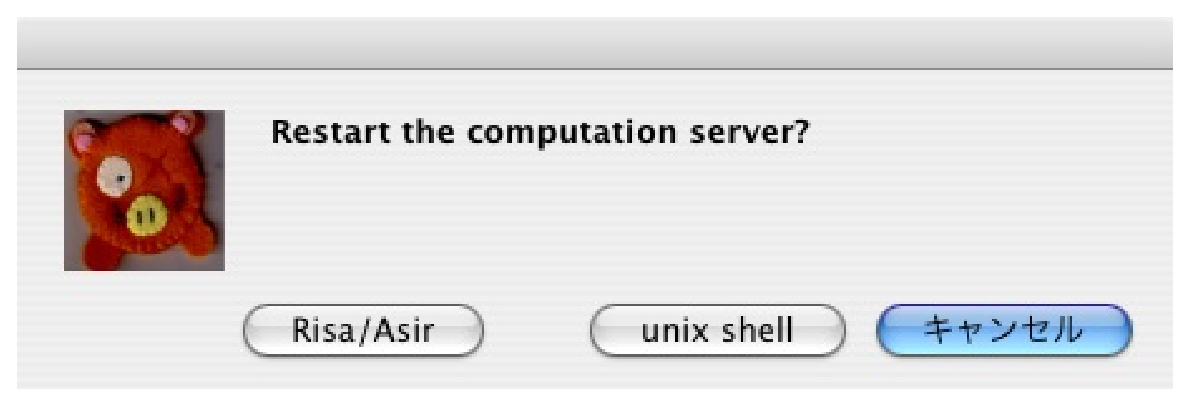
\includegraphics{Figs/restartDialog}}
\end{center}
にもあるように, 別の計算エンジンを起動することも可能である.
この例では unix shell も起動できる.

また, ``実行'' メニューから ``エンジンを自動スタートしない'' モードを選んでる
場合に計算エンジンを手動でスタートするには, このボタンを用いる.

\bigbreak

\noindent
\HHH
cfep は  \index{cfep}
Cocoa FrontEnd view Process 
の略である.
cfep は Objective C という言語および xcode 2 という開発環境を用いて
Cocoa というフレームワークのもとで開発されている.
cfep の Objective C のプログラムの一部をみてみよう.
\begin{screen}
\begin{verbatim}
  for (i=0; i<oglCommSize; i++) {
    gc = [oglComm objectAtIndex: i];
    [self execute: gc];
  }
\end{verbatim}
\end{screen}
asir と同じような {\tt for} 文があるね.

\section{ヘルプの利用}

\index{かんすう@関数}
Cfep/asir での ``関数'' とは数学の関数のように引数を与えると計算して値をもどし,
かつある仕事(表示等)をする手続きの集まりである.
例えば {\tt print}, {\tt deval}, {\tt sin}, {\tt fctr} 等は関数である.
関数を自分で定義することも可能である. これについては後の説明および
``asirドリル''を参照.

あらかじめ定義ずみの関数を ``組み込み関数'' とよぶ.
\index{help}  
\index{へるぷ@ヘルプ}  \index{くみこみかんすう@組み込み関数}
組み込み関数の詳しい説明を調べるには
``cfep のヘルプ'' から
\begin{center}
\scalebox{0.3}{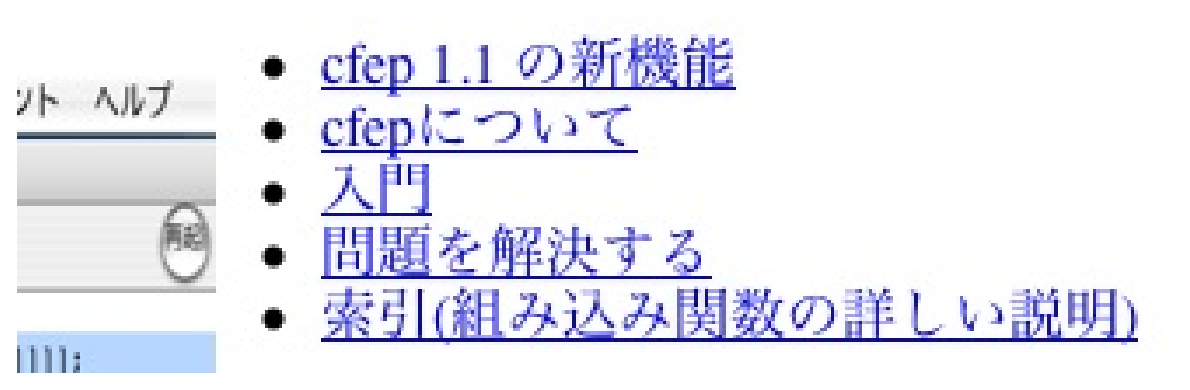
\includegraphics{Figs/helpTop}}
\end{center}
の ``索引'' を選び, 索引
\begin{center}
\scalebox{0.45}{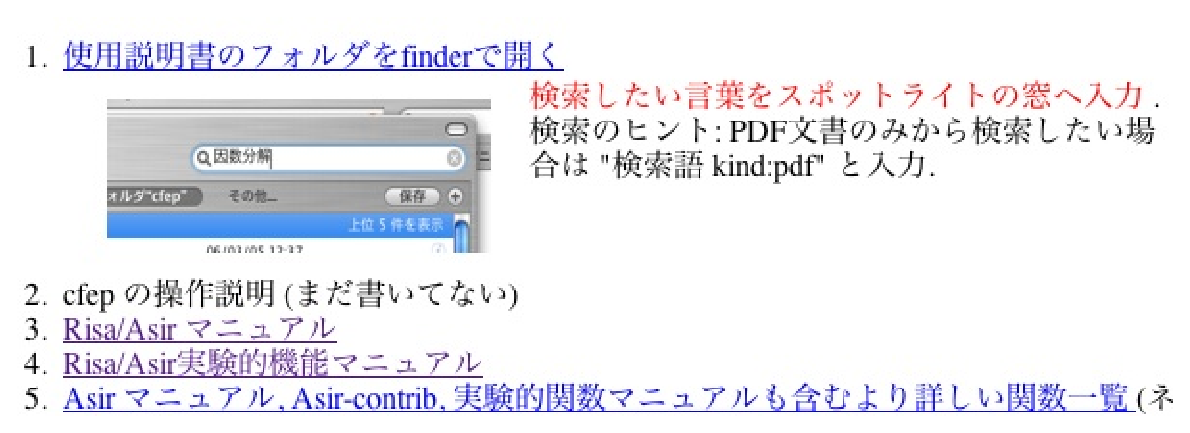
\includegraphics{Figs/helpIndex}}
\end{center}
の ``Risa/Asir マニュアル'' を選び,
``Risa/Asir マニュアル'' の最初のページの関数一覧から
調べたい関数を探す.
たとえば {\tt fctr} (因数分解用の関数) はこの一覧の中にある.
\begin{center}
\scalebox{0.35}{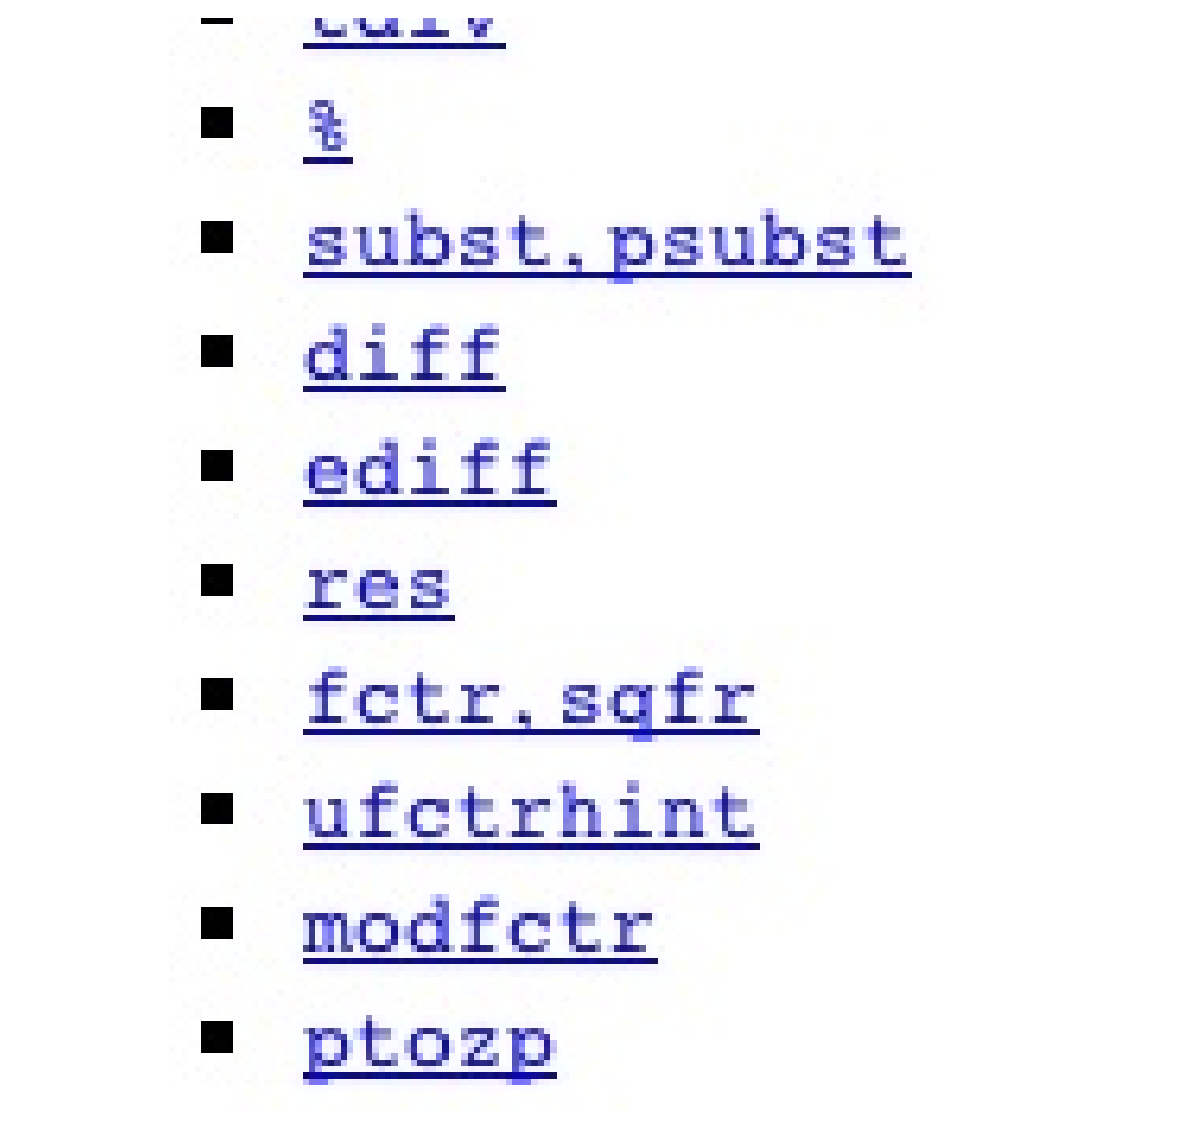
\includegraphics{Figs/helpFctr}}
\end{center}
\index{fctr}


\index{spotlight}
検索には spotlight の活用も有益であろう. 索引
\begin{center}
\scalebox{0.45}{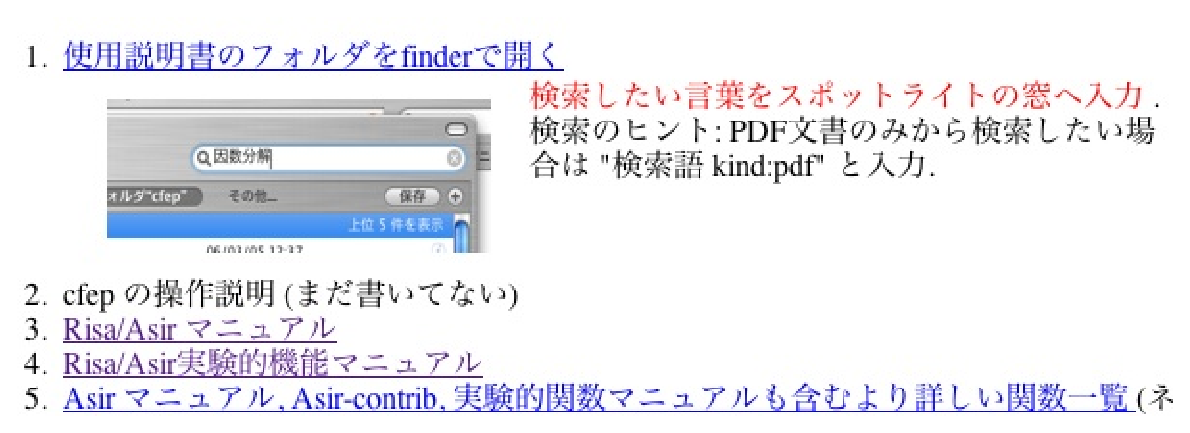
\includegraphics{Figs/helpIndex}}
\end{center}
の ``使用説明書のフォルダをfinderで開く''
を選ぶと使用説明書のフォルダが開くので, ここを spotlight で検索すると
いろいろな発見があるであろう.
ちなみに, この超入門や asirドリルはこのフォルダの pdf フォルダの中にある.
(なおここからの spotlight 検索は何故か遅いので, メニューバーの 
 splotlight からの検索の方がいいかもしれない.
)
%% mdfind, mdimport?


\chapter{グラフィック}

\section{ライブラリの読み込み}  \index{らいぶらり@ライブラリ}

\begin{figure}
\begin{center}
\scalebox{0.5}{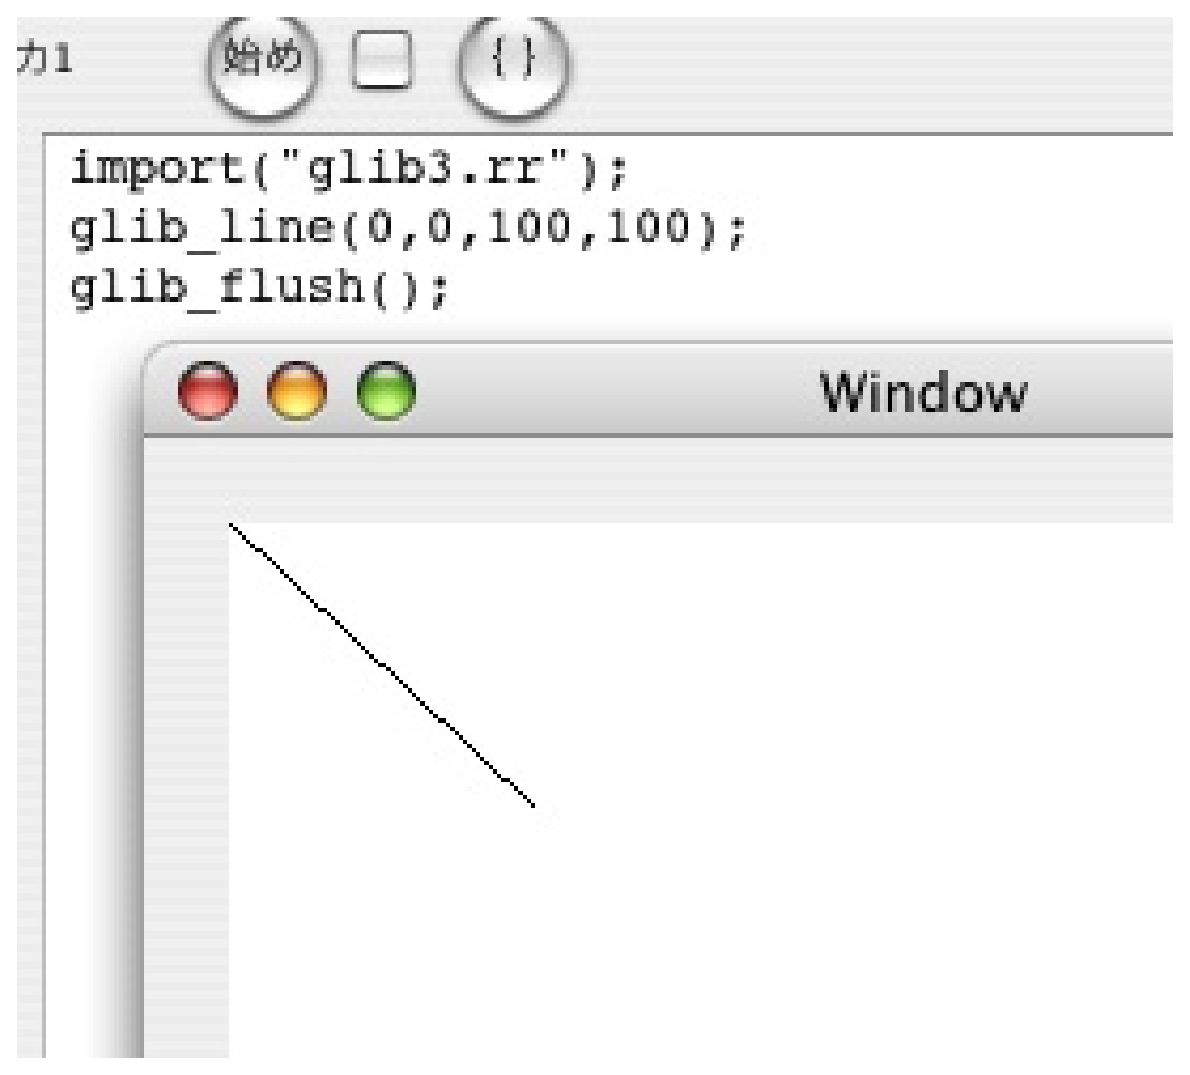
\includegraphics{Figs/glib_lineImport.eps}}
\end{center}
\caption{ライブラリのロード} \label{fig:glib_lineImport}
\end{figure}

Asir 言語で書かれている関数定義の集合がライブラリである.
ライブラリを読み込むには {\tt import} コマンドまたは
{\tt load} コマンドを用いる.   \index{import}  \index{load}
マニュアルに記述されている関数でライブラリの読み込みが前提となってるものも
多い.
たとえば, 線を引くコマンド {\tt glib\_line(0,0,100,100);} 
を実行しても, ``glib\_line が定義されていません''
というエラーが表示される.
グラフィックコマンドのライブラリ読み込むコマンド
\begin{verbatim}
  import("glib3.rr");
\end{verbatim}
を実行しておくと図\ref{fig:glib_lineImport}のように
線を描画する.


Asir-contrib プロジェクトにより集積されたライブラリの集合体が
asir-contrib である.  \index{asir-contrib}
Asir-contrib を読み込んでしまうと,
ほとんどの関数について import が必要かどうか気にする必要はなくなるが,
大量のライブラリを読み込むために時間がかかるのが欠点である.
asir-contrib は \fbox{実行} メニューから読み込める.
\begin{center}
\scalebox{0.3}{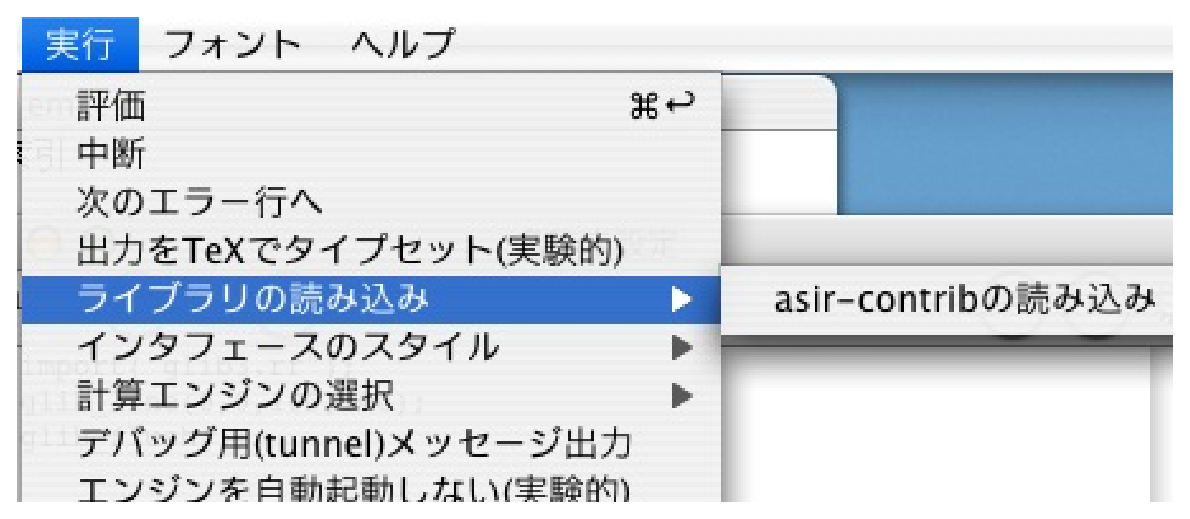
\includegraphics{Figs/importContrib}}
\end{center}

\section{線を引く関数}

\begin{example} \rm
\begin{screen}
\begin{verbatim}
   import("glib3.rr");
   glib_line(0,0, 100,100);
   glib_flush();
\end{verbatim}
\end{screen}
図\ref{fig:glib_lineImport} が描画結果である.
$y$座標は画面が下へいくほど大きくなる.
図\ref{figure:cond:coord} を参照.
左上の座標は $(0,0)$, 右下の座標が $(400,400)$.
\verb@glib_line@ で $(0,0)$ から $(100,100)$ へ線を描画.
\verb@glib_flush@ は画面を更新するはたらきがある. flush しないと,
描画結果が画面での表示に反映しない場合がある.
\end{example}

\index{glib}
{\tt glib3.rr} をロードすることにより, 次の関数が使えるようになる. \\
\begin{tabular}{|l|l|} 
\hline
{\tt glib\_window(X0,Y0,X1,Y1)} &  
                            図を書く window のサイズを決める. \\ 
 & 画面左上の座標が {\tt (X0,Y0)},
   画面右下の座標が {\tt (X1,Y1)} \\
 & であるような座標系で以下描画せよ. \\ 
& ただし x 座標は, 右にいくに従いおおきくなり, \\
&
  y 座標は \underline{下に} いくに従い大きくなる (図 \ref{figure:cond:coord}).  \\ \hline
{\tt glib\_clear()} &  全てのOpenGLオブジェクトを消去し,
                          描画画面をクリアする. \\ \hline
{\tt glib\_putpixel(X,Y)} &  座標 {\tt (X,Y)} に点を打つ. \\ \hline
{\tt glib\_set\_pixel\_size(S)} &  
   点の大きさの指定.  1.0 が1ピクセル分の大きさ. \\ \hline
{\tt glib\_line(X,Y,P,Q)} &  座標 {\tt (X,Y)} から 座標 {\tt (P,Q)} へ直線を引く \\ \hline
{\tt glib\_remove\_last()} & 一つ前の OpenGL オブジェクトを消す.  \\ \hline
\end{tabular}

\begin{figure}[htb]  
\setlength{\unitlength}{1mm}
\begin{picture}(100,40)(0,0)
\put(20,35){\vector(1,0){80}}
\put(98,32){x}
\put(20,35){\vector(0,-1){35}}
\put(23,1){y}
\end{picture}
\caption{座標系}  \label{figure:cond:coord}
\end{figure}

色を変更したいときは,  \verb@ | @ 記号で区切ったオプショナル引数
{\tt color} を使う.  \index{おぷしょなるひきすう@オプショナル引数}
たとえば,
\begin{center}
\verb@ glib_line(0,0,100,100|color=0xff0000); @
\end{center}
と入力すると, 色 {\tt 0xff0000} で線分をひく.
ここで, 色は RGB の各成分の強さを 2 桁の 16 進数で指定する.
16進数については ``asir ドリル'' を参照.
この例では, R 成分が ff なので, 赤の線をひくこととなる.
なお, 関数 {\tt glib\_putpixel} も同じようにして, 色を指定できる.
16進数を知らない人用に, 色とその16進数による表現の対応表をあげておく.

\begin{tabular}{|l|l|}
\hline 
0xffffff  & 白 \\ \hline 
0xffff00  & 黄 \\ \hline
0xff0000  & 赤 \\ \hline
0x00ff00  & 緑 \\ \hline 
0x0000ff  & 青 \\ \hline 
0x000000  & 黒 \\ \hline 
\end{tabular}

\noindent
(あとは試して下さい)

さて, 図 \ref{figure:cond:coord} で見たようにコンピュータプログラムの
世界では, 画面の左上を原点にして, 下へいくに従い, $y$ 座標が増えるような
座標系をとることが多い.
数学のグラフを書いたりするにはこれでは不便なことも多いので,
{\tt glib3.rr} では,
\begin{center}
  \verb@ Glib_math_coordinate=1; @
\end{center}
を実行しておくと 
画面の左下が原点で, 上にいくに従い $y$ 座標が増えるような
数学での座標系で図を描画する.

\begin{example} \rm   \index{ぐらふ@グラフ}
2次関数 $y=x^2-1$ のグラフを書いてみよう.
%%Prog: cfep/tests/2006-03-11-graph2d.rr
\begin{screen}
\begin{verbatim}
import("glib3.rr");
Glib_math_coordinate=1;
glib_window(-2,-2, 2,2);

glib_line(-2,0,2,0 | color=0x0000ff);
glib_line(0,-2,0,2 | color=0x0000ff);
for (X=-2.0; X< 2.0; X = X+0.1) {
   Y = X^2-1;
   X1 = X+0.1;
   Y1 = X1^2-1;
   glib_line(X,Y, X1,Y1);
}
glib_flush();
\end{verbatim}
\end{screen}
実行結果は図\ref{fig:graph2d}.
-----プログラムの解説はまだ書いてない.
\end{example}

%<C
\begin{figure}[tb]
\scalebox{0.6}{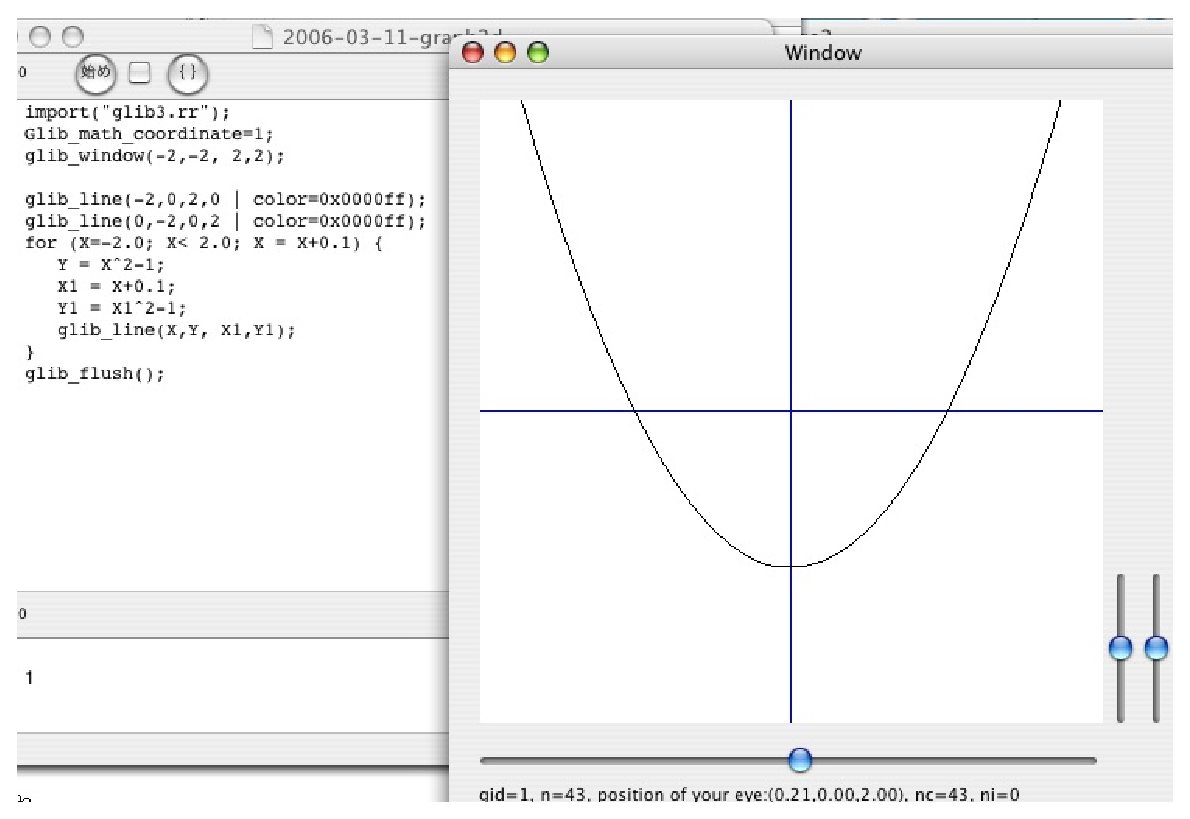
\includegraphics{Figs/graph2d.eps}}
\caption{2次関数のグラフ} \label{fig:graph2d}
\end{figure}
%>C


\section{円を描く関数を作ってみよう}

%%Prog: cfep/tests/2006-03-11-circle.rr
\begin{screen}
\begin{verbatim}
import("glib3.rr");
Glib_math_coordinate=1;
glib_window(-1,-1,1,1);
glib_clear();
E = 0.2;  X = 0; Y = 0;  R = 0.5;
for (T=0; T<=deval(2*@pi); T = T+E) {
  Px = X+deval(R*cos(T));
  Py = Y+deval(R*sin(T));
  Qx = X+deval(R*cos(T+E));
  Qy = Y+deval(R*sin(T+E));
  glib_line(Px,Py,Qx,Qy);
  glib_flush(); 
}
\end{verbatim}
\end{screen}
-----プログラムの解説はまだ書いてない.

上のプログラムでは $\cos$, $\sin$ を用いて円を描いている.
中心, 半径を変更したり, 色を変更したりしながらたくさんの円を描くには,
どのようにすればよいであろうか?
``関数'' を用いるとそれが容易にできる.

あるひとまとまりのプログラムは関数 (function) として
まとめておくとよい.   \index{かんすう@関数} 
計算機言語における関数は数学でいう関数と似て非なるものである.
関数を手続き (procedure) とか サブルーチン (subroutine) とか
よぶ言語もある.
関数を用いる最大の利点は, 関数を一旦書いてしまえば,
中身をブラックボックスとして扱えることである.
大規模なプログラムを書くときは複雑な処理をいくつかの関数に分割して
まず各関数を十分テストし仕上げる.
それからそれらの関数を組み合わせていくことにより, 
複雑な機能を実現する.
このようなアプローチをとることにより, ``困難が分割'' される.

円の例をしばらく離れ,
簡単な関数の例をとり関数の書き方を説明しよう.
前の節では $2$ の巾の表を作成するプログラムを書いた.
これを元に次のような関数を作る.
\begin{screen}
\begin{verbatim}
def power_table(N) {
  X=2;
  for (I=1; I<=N; I++) {
    print(X^I);
  }
}
power_table(8);
\end{verbatim}
\end{screen}
関数の定義は次のように {\tt def} 命令で行なう.
\begin{verbatim}
def  関数名(引数) {
  関数本体 
}
\end{verbatim}
上の例では関数名は {\tt power\_table} であり, 引数(argument)は {\tt N} である.
関数名は英数字と {\tt \_} を用いてつける.
ただし数字や大文字ではじまる名前をつけることはできない.
処理内容を連想させるような名前をつけるのが望ましい.
{\tt def} 命令では関数を定義するだけで実行は行なわない.
実行させるには, 上の例のように {\tt power\_table(8);} と引数の部分に実際の数字等を入れて
呼び出す.

引数は二つ以上あってもよくて,たとえば,
\begin{screen}
\begin{verbatim}
def power_table2(X,N) {
  for (I=1; I<=N; I++) {
    print(X^I);
  }
}
power_table2(3,8);
\end{verbatim}
\end{screen}
なる関数定義と最後の行のその呼び出しは 
$3^i$ を $i=1, \ldots, 8$ の範囲で計算して表示する.
このような関数を用意しておけば,
$2^i$, $3^i$, $5^i$, $1 \leq i \leq 10$ の表を表示したいとすると,
\begin{screen}
\begin{verbatim}
power_table2(2,10);
power_table2(3,10);
power_table2(5,10);
\end{verbatim}
\end{screen}
と書くだけで良く, プログラムも短くなり, かつ整理されているので, 読みやすくなる.

さて, {\tt power\_table2(2,3);} を実行すると
\begin{screen}
\begin{verbatim}
2
4
8
0
\end{verbatim}
\end{screen}
と表示される. 
最後の 0 は一体何であろうか?
これは実は関数の値である. 
関数の値のことを戻り値ともいう.
戻値を指定するには, {\tt return} 文を用いる.
\begin{flushleft}
\begin{minipage}[t]{7cm}
\begin{screen}
\begin{verbatim}
def twotimes(N) {
  S=2*N;
  return(S);
}
\end{verbatim}
\end{screen}
\end{minipage} \quad
%
\begin{minipage}[t]{7cm}
関数 {\tt twotimes(N)} は
$2N$ の値を計算して戻す. \\
この定義を書いておいて
\begin{verbatim}
A=twotimes(10);
B=twotimes(100);
print(A+B);
\end{verbatim}
を実行すると, {\tt A} には $20$ が代入され, {\tt B} には $200$ が代入され,
{\tt print}文により $220$ が出力される.
そのあと $0$ が出力されるがこれは {\tt print}文の戻り値である.
\end{minipage} \\
\end{flushleft}

\noindent  
関数の戻り値 (return value) は {\tt return} 文で
指定する.
いまの場合は変数 {\tt S} の値である.
なお, {\tt print} と {\tt return}  は違う.
{\tt print} は画面に値を印刷するのに対して,
{\tt return} は関数の値を戻す働きを持つ.
{\tt print} 文では, 関数の値を戻すことはできない.

``戻り値''(return value) という言い方は計算機言語特有の言いまわしである.
``関数 {\tt twotimes} は引数の2倍を計算して結果を戻す'' みたいに使う.
上の例でいえば {\tt A=twotimes(10)} としたとき,
戻り値が関数の値として変数 {\tt A} に代入される.


関数のなかで利用されている変数と引数は,
その関数の実行中のみ生成される変数であり,
さらにその関数外部の同名の変数の値を変えない.
このように一時的に生成される変数を局所変数 (local variable) とよぶ.
関数の中で変数の値を変更したら, その関数の外の同じ名前の変数の
値もかわってしまうとしたら, 処理を分割した利点がすくない.
そこででてきた概念がこの ``局所変数''
の概念である.
上のプログラム例では,
{\tt N}, {\tt S} が局所変数である.
局所変数はその関数のなかだけで有効な変数である.
これを, ``局所変数のスコープはその関数のなかだけ'' という
言いかたをする. 
局所変数の考え方は, 計算機言語の歴史では大発明の一つである.

\noindent
例:
%%%%%%%%%%  mini page template %%%%%%%%%%%%
\begin{flushleft}
\begin{minipage}[t]{7cm}
\begin{screen}
\begin{verbatim}
S=3;
twotimes(2);
print(S);
\end{verbatim}
\end{screen}
\end{minipage} \quad
%
\begin{minipage}[t]{7cm}
このプログラムの {\tt S} と関数 {\tt twotimes} のなかの変数  {\tt S} は別物
である.
したがって, {\tt twotimes} の終了時点で関数 {\tt twotimes} のなかの変数 {\tt S}
の値は $6$ であるが,  {\tt print} 文で {\tt S} の値を表示させてみても
やはり $3$ のままである.
\end{minipage} \\
\end{flushleft}


%<C
\begin{figure}[tbh]
\scalebox{0.6}{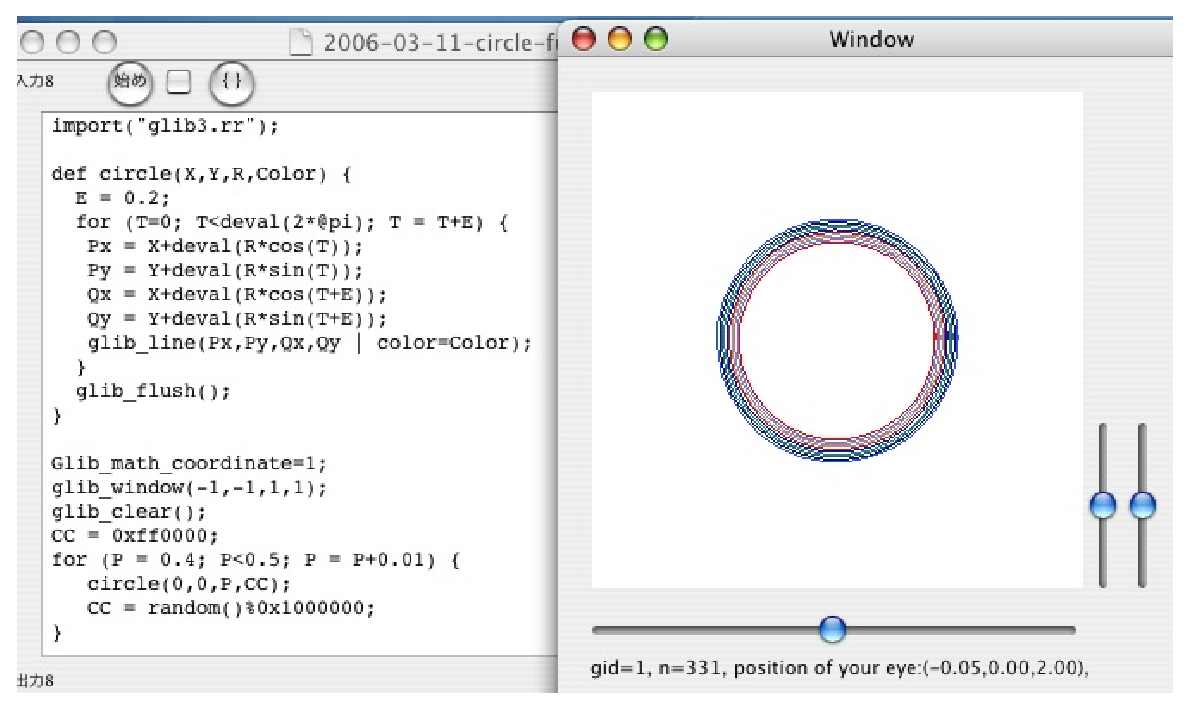
\includegraphics{Figs/circleFunc.eps}}
\caption{ 関数による同心円の描画} \label{fig:circleFunc}
\end{figure}
%>C

さて円を描く例にもどろう.
以下のように関数 {\tt circle(X,Y,R,Color)}を定義 ({\tt def}) する.
この関数を $R$ や $Color$ を変化させながら呼ぶことにより,
図\ref{fig:circleFunc} のような同心円の図を描くことが可能となる.
関数についてさらに詳しくは ``asir ドリル'' を参照してほしい.

\begin{screen}
\begin{verbatim}
import("glib3.rr"); 

def circle(X,Y,R,Color) {
  E = 0.2;  
  for (T=0; T<deval(2*@pi); T = T+E) {
   Px = X+deval(R*cos(T));
   Py = Y+deval(R*sin(T));
   Qx = X+deval(R*cos(T+E));
   Qy = Y+deval(R*sin(T+E));
   glib_line(Px,Py,Qx,Qy | color=Color);
  }
  glib_flush();
}

Glib_math_coordinate=1;
glib_window(-1,-1,1,1);
glib_clear();
CC = 0xff0000;
for (P = 0.4; P<0.5; P = P+0.01) {
   circle(0,0,P,CC);
   CC = random()%0x1000000;
}
\end{verbatim}
\end{screen}
{\tt (Qx,Qy)} と {\tt (Px,Py)} は
{\tt E} だけ偏角が異る.
円を多面体で近似して描画している. \\
-----プログラムの詳しい解説まだ.

\begin{problem} \rm
\begin{enumerate}
\item このプログラムの関数を用いて接する半径の同じ円を二つ描画するプログラムを書きなさい.
\item 円を塗り潰す関数を作れ.
\item 分度器を描くプログラムを作れ.
\item (発展課題) この分度器, 糸, おもり, わりばし, 板, cfep/asir によるプログラム等を用いて,
木やビルの高さを測定する機械とソフトウエアシステムを開発せよ.
\end{enumerate}
\end{problem}

\begin{problem} \rm
(これは発展課題)  \index{OpenGL}  \index{3じげんぐらふぃっくす@3次元グラフィックス}
cfep には OpenGL インタプリターが組み込んである.
OpenGL は3次元グラフィックスを用いるソフトウエア作成のために
用いられる約 150種類のコマンドから構成されているパッケージで
3次元グラフィックスの標準規格のひとつでもある.
cfep 1.1ではその中の 10 弱のコマンドを利用できる.

この OpenGL インタプリターを用い,
多面体(polygon)を材料にし,
cfep上級編, OpenGL のプログラムを参考に
``家'' を書いてみよう. 
\end{problem}


\noindent
\fbox{\bf 実習の落とし穴}\\
\begin{enumerate}
\item unix 版, windows 版では asir ドリルにあるように
\verb@ end$ @ %$
をプログラムの最後に書かないと行けないが, cfep/asir ではこの命令は
計算エンジンの停止命令となるので書いてはいけない.
ただし\underline{行の頭}に\underline{空白をいれずに}書いてある 
\verb@ end$ @ %$
は自動削除されるので, unix, windows 版共通のプログラムを書くときは
空白を入れずに行の頭に書いておくと便利である.
\item 空白や改行は原則自由に挿入していいが, 空白を入れてはいけない表現がある.
たとえば
\begin{verbatim}
0.1
\end{verbatim}
と書くべきところを
\begin{verbatim}
0. 1
\end{verbatim}
と $1$ の前に空白を入れるとエラーとなる. 
数字には空白を入れてはいけない.
理由は asir ドリルの構文解析の章を読むと理解できると思う.
\item {\tt sin\ x} なる表現は受け付けてくれない. 
必ず括弧がいる. つまり {\tt sin(x)} と書く.
\item 掛け算の {\tt *} は省略できない.
\end{enumerate}

\noindent
\HHH.
{\tt [1,2,3]} のように {\tt []} で囲った表現をリスト(list)と呼ぶ.
関数の戻り値を数の組にしたいときはリストを値として戻すと良い.
{\tt print} 文で多くの数を一行で表示したいときもリストを使うと便利である.
{\tt L} をリストとするとき {\tt L[0]} でリストの最初(0番目)の元,
{\tt L[1]} でリストの1番目の元, ... を表す. 
詳しくは asir ドリル参照.
\begin{screen}
\begin{verbatim}
L=[3,2,1];
print(L);
print(L[0]+L[1]+L[2]);
\end{verbatim}
\end{screen}
%%Note: misc-2010/10/keisan-1/note-ja.txt  講義の進度.

\chapter{For 文による数列の計算}

\section{超入門, 第2の関門: 漸化式できまる数列の計算}

\begin{example} \rm
$a$ を正の数とするとき,
\begin{eqnarray*}
  x_{n+1} &=& \frac{x_n + \frac{a}{x_n}}{2}, \\
  x_0 &=& a
\end{eqnarray*}
できまる数列 $x_0, x_1, x_2, \ldots $ 
は $\sqrt{a}$ にどんどん近付くこと(収束すること)が知られている.
$a=2$ の時, $x_1, x_2, \ldots, x_4, x_5$ を計算するプログラムを書いてみよう.
%%Prog: cfep/tests/2006-03-11-sqrt.rr
\begin{screen}
\begin{verbatim}
A = 2.0;
X = A;
for (I=0; I<5; I++) {
  Y = (X+A/X)/2; 
  print(Y);
  X = Y;
}
\end{verbatim}
\end{screen}
\end{example}

このプログラムの実行結果は図\ref{fig:sqrt}.
%<C
\begin{figure}[tbh]
\scalebox{0.5}{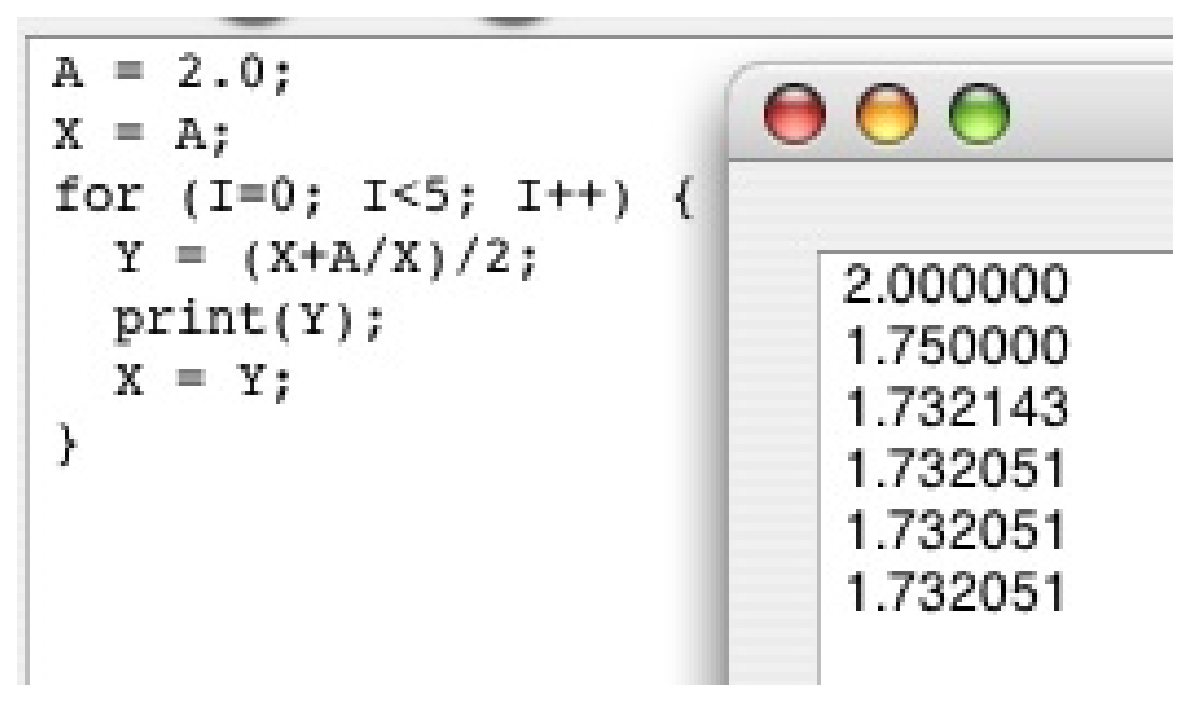
\includegraphics{Figs/sqrt.eps}}
\caption{$\sqrt{2}$ に収束する数列} \label{fig:sqrt}
\end{figure}
%>C

超入門での関門は
\begin{screen}
\begin{verbatim}
  Y = (X+A/X)/2; 
  X = Y;
\end{verbatim}
の意味を完全に理解すること
\end{screen}
である.
変数の章で説明したように, 
$$  \mbox{{\bf 変数名}} {\tt = }  \mbox{{\bf 式}} {\tt  ;} $$
はまず右辺の式を計算しそのあとその計算結果を左辺の変数に代入せよという意味
である. したがって,
\verb@  Y = (X+A/X)/2;  @ は現在の {\tt X} と {\tt A} に格納された
数字をもとに \verb@ (X+A/X)/2 @ の値を計算し, その結果を変数 {\tt Y} へ代入せよ,
という意味である. また
\begin{screen}
\verb@X=Y@ は \verb@X@ が \verb@Y@ に等しいという意味ではなく,
変数\verb@Y@ に格納された数字を 変数 \verb@X@ に代入せよという意味である.
\end{screen}
このように考えれば, 上のプログラムが $x_1, x_2, x_3, x_4$ の値を
順番に計算して print している理由が理解できるであろう.
自分が計算機になったつもりで,
変数の中の数値がどのように変化していくのか,
書きながら理解して頂きたい.
これがはっきり理解でき, 応用問題が自由に解けるようになった, 超入門卒業である.
\index{だいにゅう@代入}

\begin{problem} \rm
変数 {\tt I}, {\tt X}, {\tt Y} の値は {\tt for} ループ内でどのように
変化するか?
{\tt Y= (X+A/X)/2} の行が実行される前のこれらの変数の値を表にして
まとめよ.  {\tt print([I,X,Y])} をはさむことによりこの表が正しいことを
たしかめよ.
\end{problem}
表は次のような形式で書く.
\begin{tabular}{|c|c|c|c|c|c|}
\hline
{\tt I} & 0&1&2&3&4 \\ \hline
{\tt X} & &&&& \\ \hline
{\tt Y} & &&&& \\ \hline
\end{tabular}

\begin{problem} \rm
プログラムのバグ(bug)とはなにか? 
\end{problem}

\section{円を描く数列}

前の章で円を描く関数を紹介した.
$\sin$,$\cos$ の計算に時間がかかる計算機では, なるべく
これら三角関数を用いないで円を描画する必要がある.

一つの方法は $s=\tan \frac{t}{2}$ とおくと
$\cos t = \frac{1+s^2}{1-s^2}$,
$\sin t = \frac{2s}{1-s^2}$
と書けるという公式を使う方法である.
$s$ はタンジェントで定義されていることを忘れてしまえばよい.  

もう一つは
数列の計算を用いて, $\cos$ や $\sin$ の計算をやらずに円を描く
方法である.
%%Prog: cfep/tests/2006-03-11-circle-dda.rr
\begin{screen}
\begin{verbatim}
import("glib3.rr");
Glib_math_coordinate=1;
glib_window(-2,-2, 2,2);
glib_clear();
E = 0.1;   
C1 = 1.0; C2=1.0;
S1 = 0.0; S2=E; 
for (T=0; T<=deval(2*@pi); T = T+E) {
    C3 = 2*C2-C1-E*E*C2;
    S3 = 2*S2-S1-E*E*S2;
    glib_line(C1,S1, C2,S2); 
    C1=C2; S1=S2;
    C2=C3; S2=S3;
    glib_flush(); 
}
\end{verbatim}
\end{screen}

このプログラムの実行結果は図\ref{fig:circleDda}.
%<C
\begin{figure}[tbh]
\scalebox{0.6}{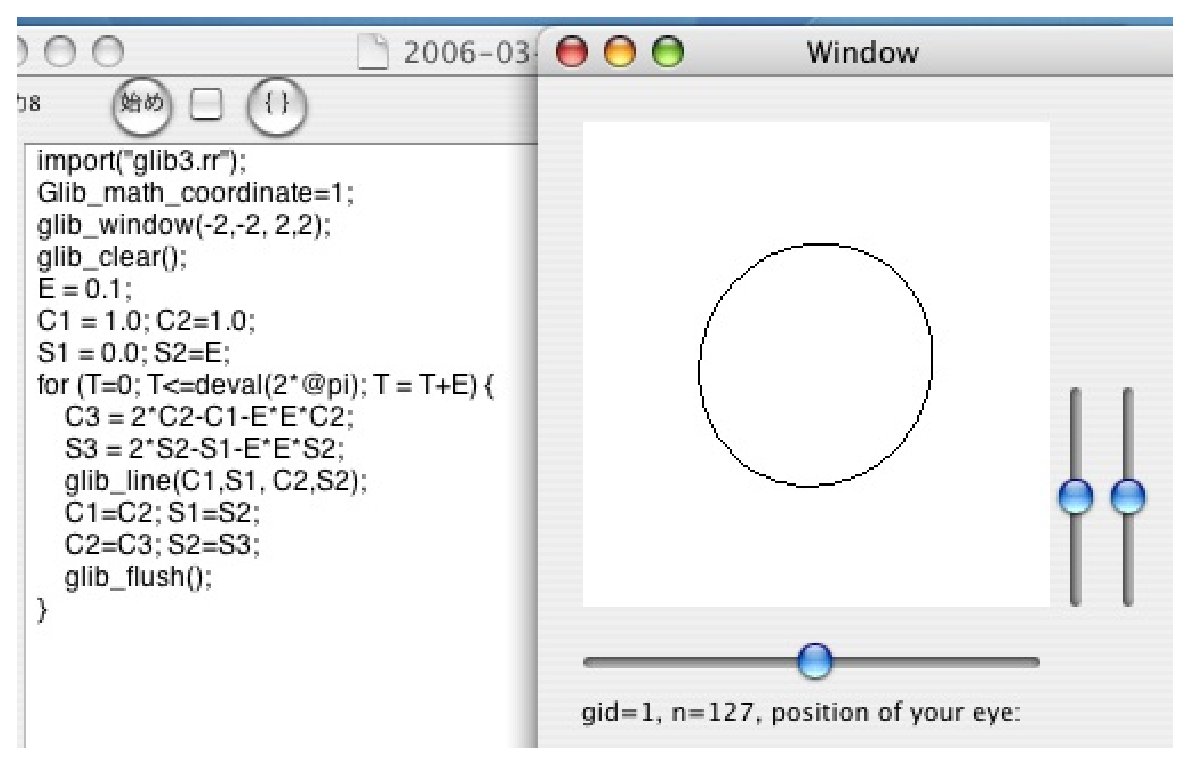
\includegraphics{Figs/circleDda.eps}}
\caption{$\cos$, $\sin$ を使わずに円を描く} \label{fig:circleDda}
\end{figure}
%>C

-----プログラムの解説まだ書いてない.

ヒント: 
微分方程式 $d^2 x/dt^2 = -x, d^2 y/dt^2 = -y$ を $t$ をラジアンとして
差分法で近似的に解いている.

この話題は, 数列の計算と差分方程式によるシミュレーションに続く.
これについてはまた稿をあらためて書いてみたい.

以上で超入門は終了である.  続きは ``Asir ドリル'' を読んでね. 
特に配列と関数をマスターすると数学プログラムには重宝する.

なお, asir ドリルに紹介してあるプログラムは \verb@ end$ @  %$
または \verb@ end; @ が最後に書いてある場合が多いが,
cfep/asir ではこの {\tt end} を書いてはいけない.
{\tt end } は計算エンジンの停止命令であり, 実行されると ``計算中の表示'' がでて無応答となる.
(一応, 行頭にあるこれらの命令は自動的に削除するようになってはいる.)
%% kxx/ox_texmacs.c

\begin{problem} \rm
(レポート問題の例) \\
なにか図を描くプログラムを書きなさい. (定番ドラエモンでもよい)
\end{problem}

\noindent
\fbox{ノート}.
著者の場合, 週に1コマ講義, 演習1コマでは, ここまでで3週である.
上のレポート問題が最初のレポート.
3週目の演習の時間からとりかかり, 5週目の演習の時間に発表.
4週目からは asirドリル.

\chapter{cfep 上級編}

\section{\TeX によるタイプセット(実験的)}
%%Doc: cfep/tests/2006-03-06
出力をTeXでタイプセットするには 
``実行'' メニューから ``出力をTeXでタイプセット'' を選択する.
{\tt latex}, {\tt dvipng} がインストールされてい
ないと動作しない.
これらはたとえば {\tt fink}  から \TeX をインストールしたり,
{\tt ptex\_package\_2005v2.1.dmg} (最近の状況は ptex package macosx で検索)
などで Mac 用の pTeX をインストールしておけばよい.
\TeX を用いた仕上り例は図\ref{fig:sl2}を見よ. 
なお, \TeX でタイプセットする場合ホームの下に
\verb@OpenXM_tmp@ なる作業用のフォルダが作成される.
タイプセットは実験機能のため, このフォルダの中の作業用ファイルは自動では消去されない.
時々手動で作業ファイルを消去されたい.
\index{tex@\TeX}

\section{選択範囲のみの実行}

\index{せんたくはんいのみのじっこう@選択範囲のみの実行}
画面上の ``選択範囲のみを実行'' をチェックすると,
``始め'' ボタンをおしたとき, 選択範囲のみが評価される.
選択範囲がない場合はキャレット位置の行が自動選択されて実行される.
\command{{\tt Enter}} と組み合わせてこの機能を使うと, ターミナルから 
asir を利用するのにちょっと似てくる.
図\ref{fig:sl2}はこのような実行をしている例である.

%<C
\begin{figure}[tbh]
\scalebox{0.5}{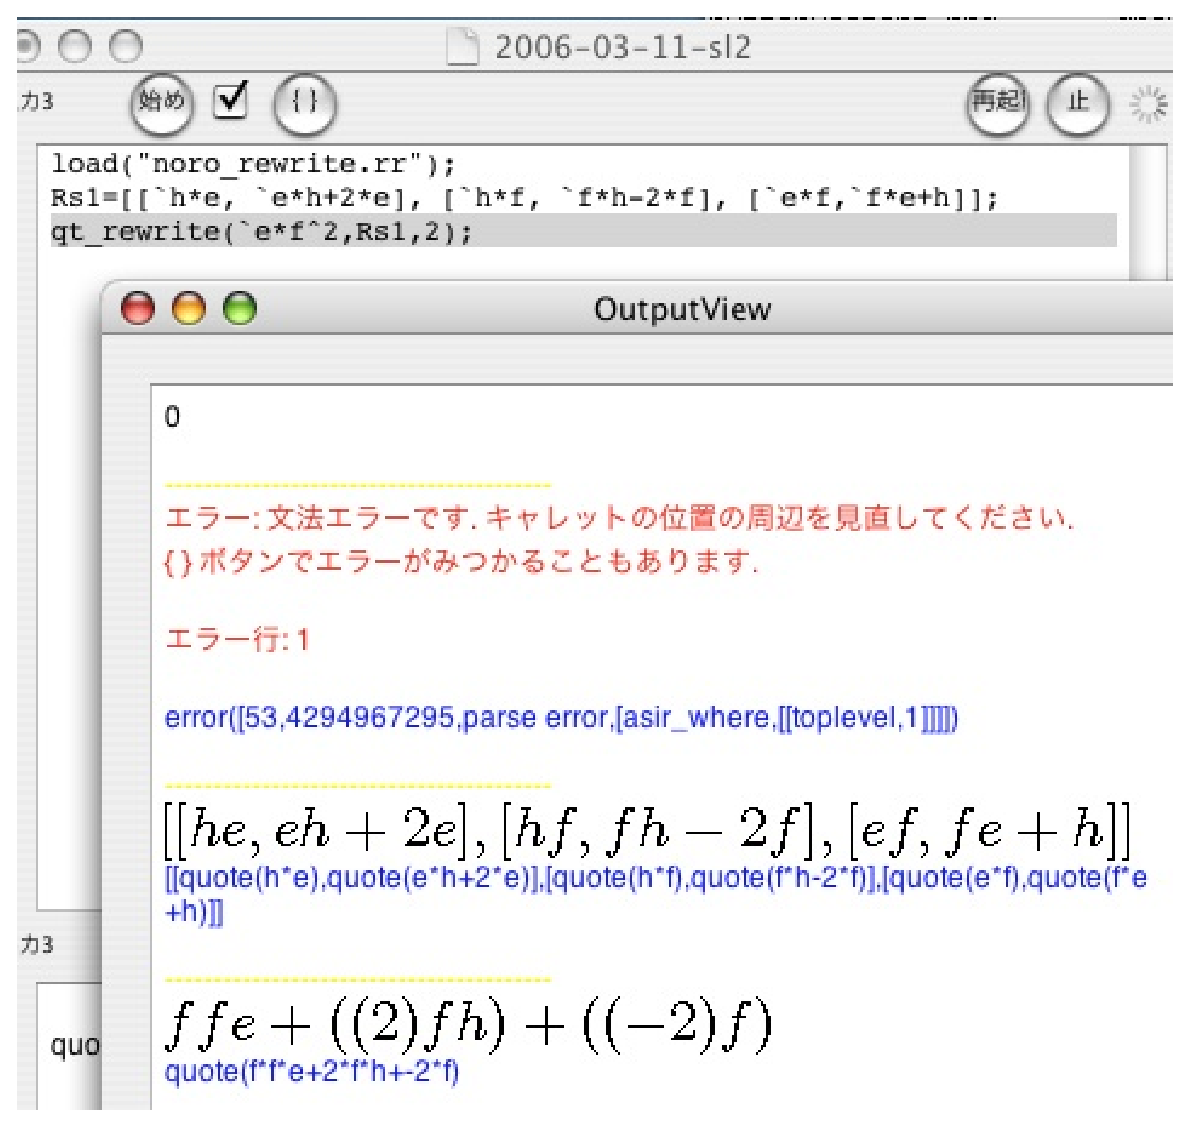
\includegraphics{Figs/sl2.eps}}
\caption{ターミナル風} \label{fig:sl2}
\end{figure}
%>C


\noindent
%%Doc:  cfep/tests/2007-03-07-debug.rtfd
\fbox{質問}
cfep のインタフェースでデバッグをしながらプログラムを開発するにはどのようにやると
よいか? \\
\fbox{答え}
cfep は初心者向きのインタフェースなので,
大規模なプログラム開発を想定していないが, 
私は次のようにライブラリの開発をしている.

\begin{enumerate}
\item 必要な関数を書く. 下の例では {\tt sum1}.
\item 関数をテストする入力をコメントの形でその関数の近くに書いておく.
下の例ではコメントにある {\tt sum1(10,1); } 等.
\end{enumerate}


\begin{screen}
\begin{verbatim}
/*
testinput:  sum1(10,1);
testinput:  sum1(10,2);
*/
def sum1(N,M) {
  S = 0; i=1;
  for (I=1; I<N; I++) {S = S+I^M; }
  return S;
}
\end{verbatim}
\end{screen}

\begin{enumerate}
\item ``始め'' ボタンで関数定義をロード. 
この時点で文法エラーなどがあればメッセージにしたがって修正.
\item そのあと ``選択範囲のみを実行'' のモードに変更してコメント内の testinput を実行.
\item 実行時のエラーの行番号への移動は "選択範囲のみを実行" のモードを解除してから
行う.   \index{えらー@エラー}
\end{enumerate}

%<C
\begin{figure}[tb]
\scalebox{0.5}{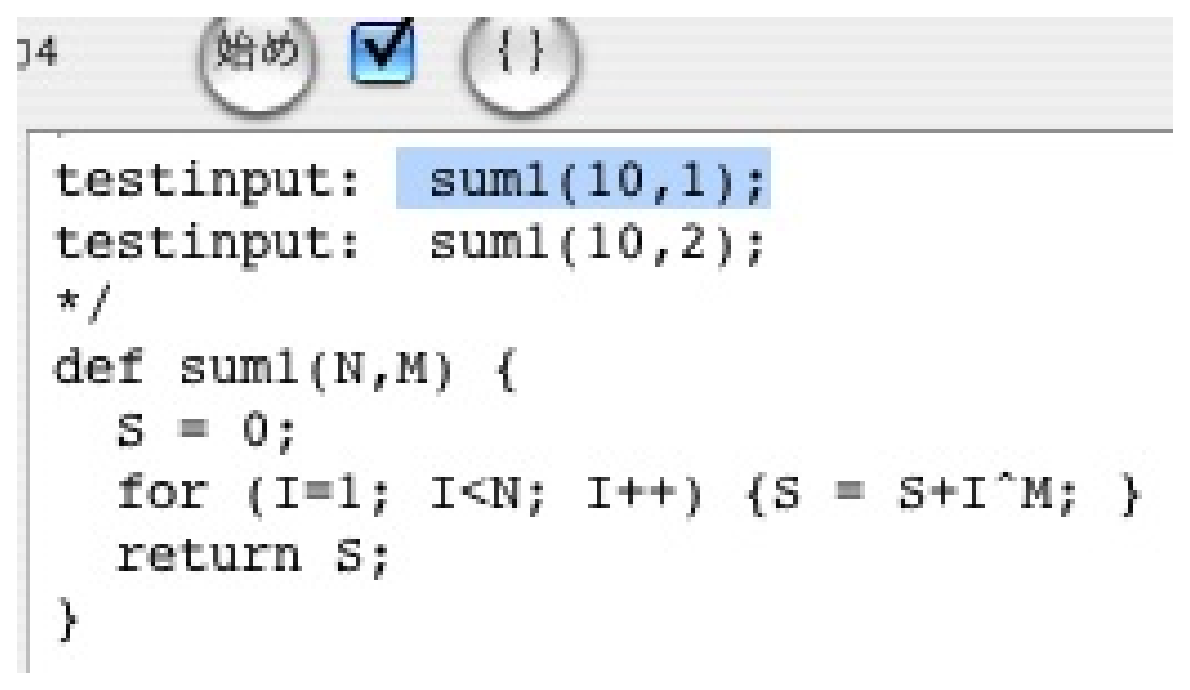
\includegraphics{Figs/howtoDebug1.eps}}
\caption{``選択範囲のみを実行''の活用} \label{fig:howtoDebug1}
\end{figure}
%>C


\section{エンジンを起動しない}
%%cfep/tests/2006-03-08-noEngine

\noindent
\fbox{質問}
 テキスト編集またはテキストの閲覧だけで計算をするつもりはありませんが. \\
\fbox{答え} 
   ``実行'' メニューで ``エンジンを自動起動しない'' を選択. \\
%<C
\scalebox{0.3}{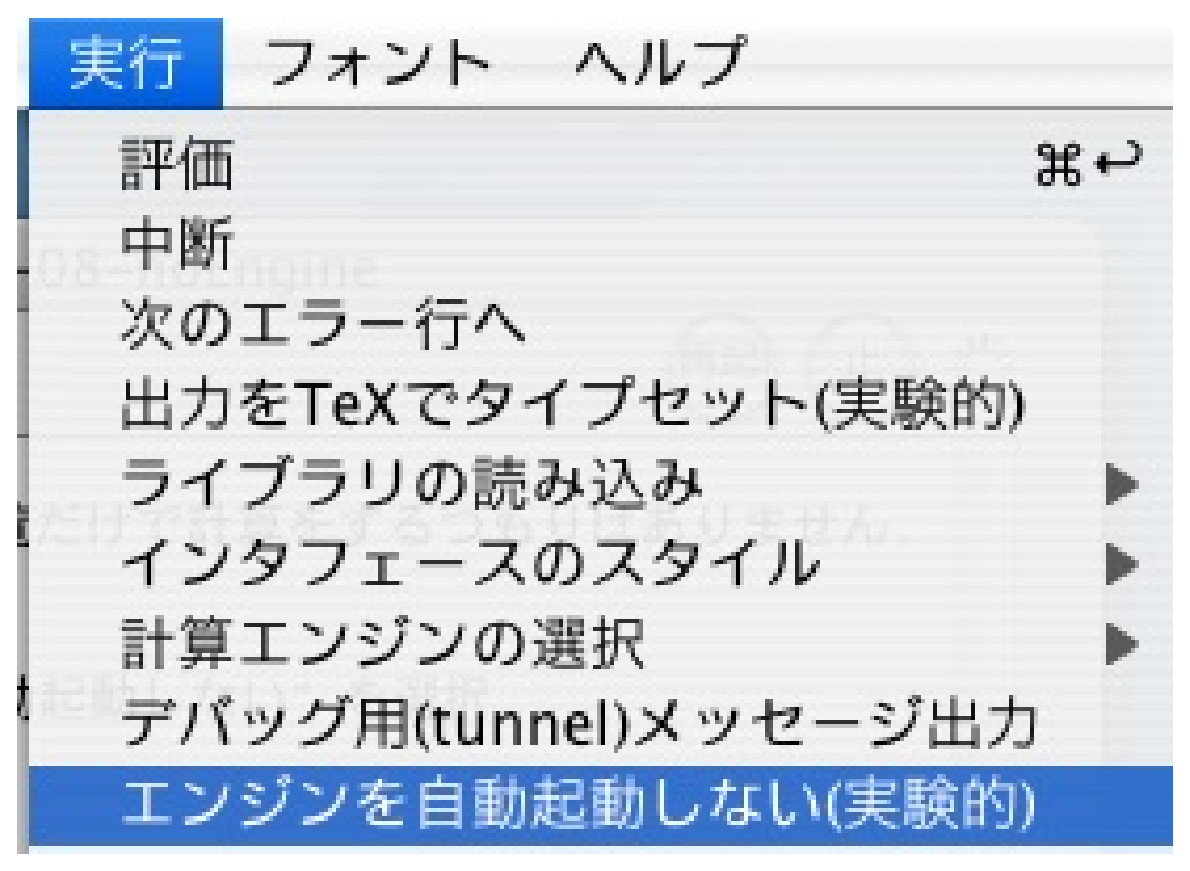
\includegraphics{Figs/menuNoEngine.eps}} \\
%>C
あとでエンジンを起動したい場合は  ``再起'' ボタンをおしてエンジンを起動する. \\
%<C
\scalebox{0.3}{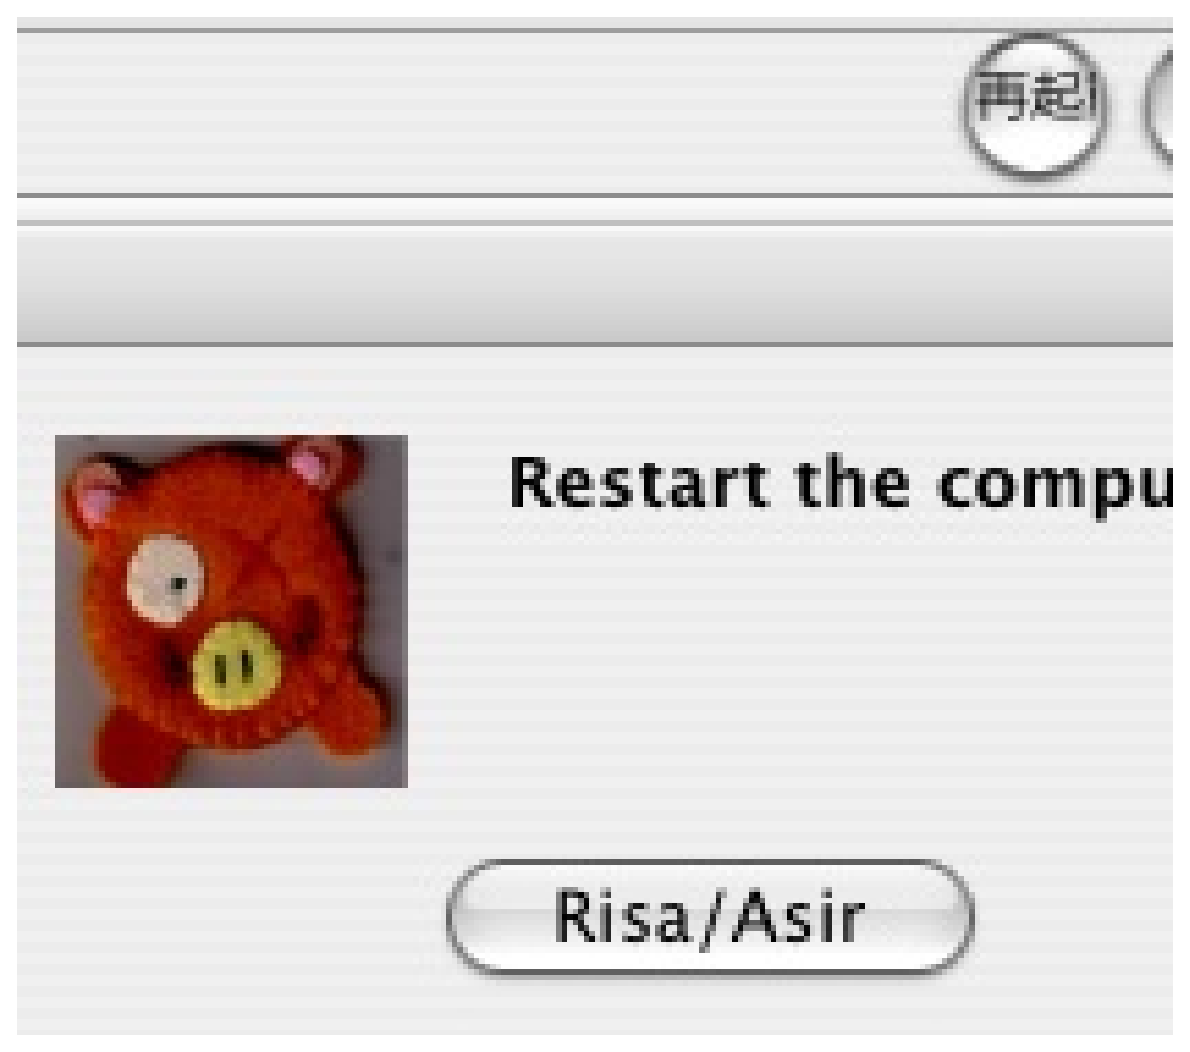
\includegraphics{Figs/popupRestart.eps}}
%>C


\section{OpenGLインタプリタ}

\index{OpenGL}
Cfep には OpenGL インタプリターが組み込んである
\footnote{{\bf 注意}: cfep/asir の
OpenGL は MacOS 10.13 (High Siera) 以降では動作しない.
glib も X11 を用いている.}.
OpenGL は3次元グラフィックスを用いるソフトウエア作成のために
用いられる約 150種類のコマンドから構成されているパッケージで
3次元グラフィックスの標準規格のひとつでもある.
cfep 1.1ではその中の 10 弱のコマンドを利用できる.
詳しくは
{\tt cfep.app/OpenXM/lib/asir-contrib/cfep-opengl.rr} を参照.

\index{OpenGLぐらふぃっくおぶじぇくと@OpenGLグラフィックオブジェクト}
OpenGL ではまず OpenGLグラフィックオブジェクトを配置し,
それから視点の位置から見た画像を描画する方法を用いる.
したがって, システムは常に OpenGLグラフィックオブジェクトの集合を保持
している.
{\tt glib\_remove\_last()} 命令はその最後の要素を削除する命令である.
{\tt cfep-opengl.rr} ライブラリでは,
{\tt opengl.metaRemoveLast()} 関数で最後の要素を削除できる.
\index{opengl}

%<C
\begin{figure}[tb]
\scalebox{0.6}{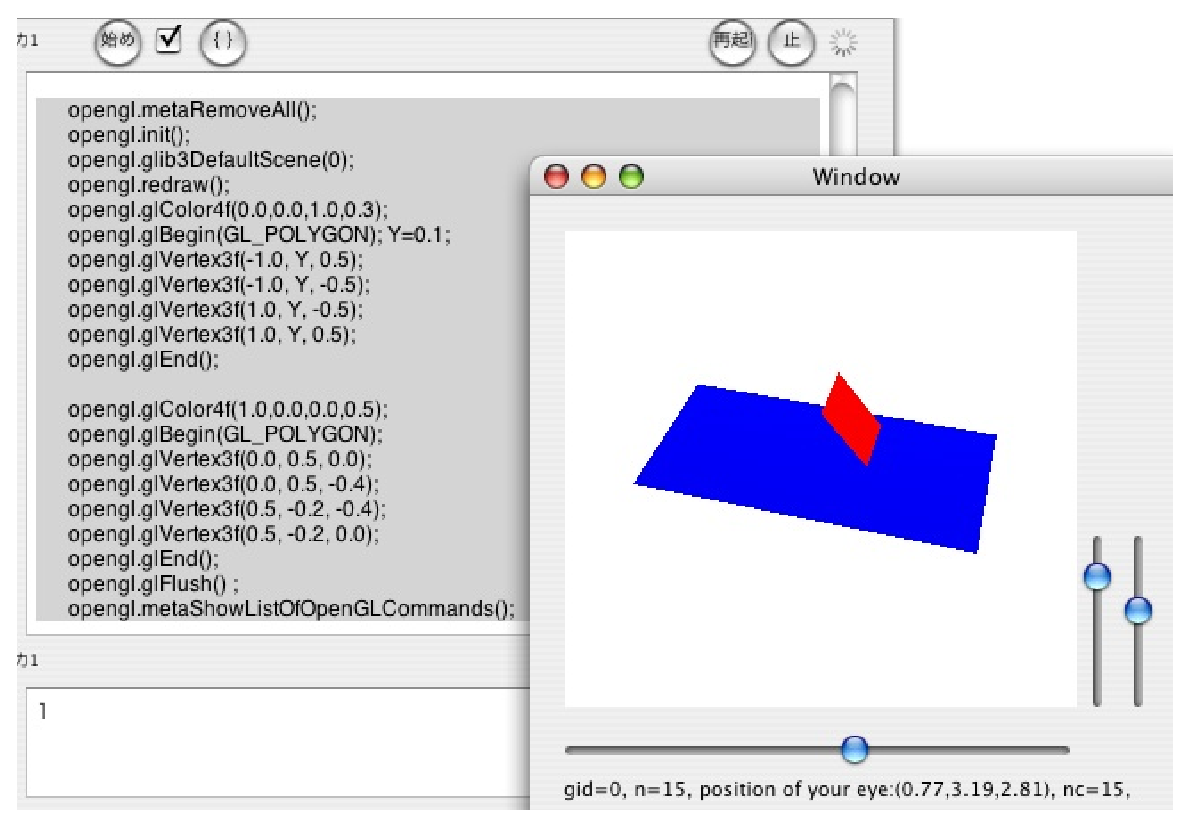
\includegraphics{Figs/twoPolygon.eps}}
\caption{} \label{fig:twoPolygon}
\end{figure}
%>C

\begin{screen}
\begin{verbatim}
      import("cfep-opengl.rr");
      opengl.metaRemoveAll();
      opengl.init();      
      opengl.glib3DefaultScene(0);
      opengl.redraw(); 
      opengl.glColor4f(0.0,0.0,1.0,0.3);  
      opengl.glBegin(GL_POLYGON); Y=0.1;
      opengl.glVertex3f(-1.0, Y, 0.5);
      opengl.glVertex3f(-1.0, Y, -0.5);
      opengl.glVertex3f(1.0, Y, -0.5);
      opengl.glVertex3f(1.0, Y, 0.5);
      opengl.glEnd();

      opengl.glColor4f(1.0,0.0,0.0,0.5); 
      opengl.glBegin(GL_POLYGON);
      opengl.glVertex3f(0.0, 0.5, 0.0);
      opengl.glVertex3f(0.0, 0.5, -0.4);
      opengl.glVertex3f(0.5, -0.2, -0.4);
      opengl.glVertex3f(0.5, -0.2, 0.0);
      opengl.glEnd();
      opengl.glFlush() ; 
      opengl.metaShowListOfOpenGLCommands();
\end{verbatim}
\end{screen}
このプログラムでは 2 枚の長方形を描いている.
このプログラムの出力は図\ref{fig:twoPolygon}.
-----詳しい説明はまだ.

OpenGL の画面には普通の数学のように $(x,y)$ 座標がはいっており,
画面から手前側が $z$ 座標が正の方向, 画面の向こう側が
$z$ 座標が負の方向である. 
``目'' から原点方向を見た画像が
図\ref{fig:twoPolygon}にあるように 3 つのスライダーを用いて目の位置を動かせるので,
OpenGLオブジェクトをいろいろな角度からみることが可能である.
下のスライダーが目の $x$ 座標, 右の二つのスライダーがそれぞれ目の $y$, $z$ 座標である.
目の動きに慣れるには, 次の二つのデモ画面をためすと面白いだろう.
\begin{screen}
\begin{verbatim}
import("cfep-opengl.rr");
opengl.glib3DefaultScene("mesa demo/ray");
\end{verbatim}
\end{screen}

\begin{screen}
\begin{verbatim}
import("cfep-opengl.rr");
opengl.glib3DefaultScene("cfep demo/icosahedron");
\end{verbatim}
\end{screen}

\section{asir 以外の計算エンジンの利用}

cfepから asir 以外の OpenXM 準拠の計算エンジンも利用できます.
たとえば, 実行, 計算エンジンの選択で, kan/sm1 を利用することも可能です.
cfep, {\tt ox\_texmacs}, {\tt ox\_sm1} が相互に通信しながら計算しています.

なお kan/sm1 の {\tt run} コマンドは使えません.
\begin{verbatim}
[(parse) (ファイル名)  pushfile] extension 
\end{verbatim}
で代用して下さい.

\cleardoublepage
\flushbottom
\printindex

\end{document}
